\documentclass[a4paper,12pt]{article}

\usepackage{fontspec}
\usepackage{fancyhdr}
\usepackage[pdfauthor={Yousef Raffa},pdftitle={Translation of The ARRL LoTW Registration Instructions in Arabic}]{hyperref}
	\hypersetup{
	    colorlinks=true,
	    citecolor=black,
	    filecolor=black,
	    linkcolor=gray,
	    urlcolor=gray
	}
\usepackage[depthadjust]{marginnote}
\usepackage[usenames,dvipsnames]{xcolor}
\usepackage{graphicx}
\graphicspath{ {./img/} }
\usepackage{fourier-orns}
\usepackage[showframe=false,includeheadfoot]{geometry}
	\geometry{verbose,top=5mm,headheight=20mm,headsep=10mm,hmargin=18mm,bottom=15mm,footskip=18mm,marginparsep=3mm,marginparwidth=12mm}
%	\geometry{verbose,hmargin=18mm,footskip=18mm,marginparsep=3mm,marginparwidth=12mm}
	 % \geometry{verbose,lmargin=20mm,rmargin=20mm,footskip=1cm}
\usepackage{polyglossia}
\usepackage{color}
\usepackage{transparent}
% set numerals=maghrib so page numbers are displayed in Arabic instead of
% eastern Arabic numerals. Otherwise, remove it for eastern Arabic numerals.
\setmainlanguage[numerals=maghrib]{arabic}
\setotherlanguage{english}
\setcounter{tocdepth}{3}


\setmainfont[Ligatures=TeX]{Amiri}
\setsansfont[Ligatures=TeX,Script=Arabic,Scale=1.5]{Amiri}
\setmonofont{Courier New}
\newfontfamily\arabicfont[Script=Arabic,Ligatures=TeX]{Amiri}

% Page styles and margins
% \pagestyle{headings}
\pagestyle{fancy}
% with this we ensure that the chapter and section
% headings are in lowercase.
\renewcommand{\sectionmark}[1]{%
        \markboth{#1}{}}
\renewcommand{\sectionmark}[1]{%
        \markright{\thesection\ #1}}
\fancyhf{}  % delete current header and footer
\fancyhead[LE,RO]{\bfseries\thepage}
\fancyhead[LO]{\bfseries\rightmark}
\fancyhead[RE]{\bfseries\leftmark}
\fancyfoot[L]{\bfseries\footnotesize\leafleft\href{http://www.HZ1YR.com}{HZ1YR.com}\leafright}
\renewcommand{\headrulewidth}{0.6pt}
\renewcommand{\footrulewidth}{0pt}
\addtolength{\headheight}{0.5pt} % space for the rule
\fancypagestyle{plain}{%
	\fancyhf{} % clear all header and footer fields
	\fancyhead{} % get rid of headers on plain pages
	\fancyhead[R]{
\includegraphics[height=3cm]{SAR.png}}% 
	\fancyhead[L]{\includegraphics[height=3cm]{ARRL.png}}% 
	\fancyfoot[C]{\bfseries \thepage} % except the center
	\renewcommand{\headrulewidth}{0pt}
	\renewcommand{\footrulewidth}{0pt}}

% Change the default sizes of header and footer
% \setlength{\headheight}{25pt}


% Setting newcommands
\newcommand{\HRule}{\rule{\linewidth}{0.5mm}}
\renewcommand*{\marginfont}{\color{slategray2}\sffamily}


% Setting newenvironment
% Dedication
\newenvironment{dedication}
{
   \cleardoublepage
   \thispagestyle{plain}
   \vspace*{\stretch{1}}
	\hfill\begin{minipage}[t]{0.66\textwidth}
   \raggedleft
}%
{
   \end{minipage}
   \vspace*{\stretch{3}}
	\begin{center}
		\color{slategray2}
	{\Huge\decoone}
	\end{center}
   \clearpage
}


% COLORS
\definecolor{darkgreen}{rgb}{0.4, 0.01, 0.24}
\definecolor{royalazure}{rgb}{0.0, 0.22, 0.66}
\definecolor{brown}{rgb}{0.4, 0.01, 0.24}
\definecolor{babyblueeyes}{rgb}{0.63, 0.79, 0.95}
\definecolor{unitednationsblue}{rgb}{0.36, 0.57, 0.9}
\definecolor{blue(rgb)}{rgb}{0.01, 0.28, 1.0}
\definecolor{darkblue}{rgb}{0.0, 0.0, 0.55}
\definecolor{screamingreen}{rgb}{0.46, 1.0, 0.44}
\definecolor{limegreen}{rgb}{0.2, 0.8, 0.2}
\definecolor{islamicgreen}{rgb}{0.0, 0.56, 0.0}
\definecolor{upforestgreen}{rgb}{0.0, 0.27, 0.13}
\definecolor{icterine}{rgb}{0.99, 0.97, 0.37}
\definecolor{orange(colorwheel)}{rgb}{1.0, 0.5, 0.0}
\definecolor{orange-red}{rgb}{1.0, 0.27, 0.0}
\definecolor{oucrimsonred}{rgb}{0.6, 0.0, 0.0}
\definecolor{cottoncandy}{rgb}{1.0, 0.74, 0.85}
\definecolor{orchid}{rgb}{0.85, 0.44, 0.84}
\definecolor{vividcerise}{rgb}{0.85, 0.11, 0.51}
\definecolor{patriarch}{rgb}{0.5, 0.0, 0.5}
\definecolor{lightbrown}{HTML}{BF6830}
\definecolor{gray}{HTML}{616D7E}
\definecolor{slategray2}{HTML}{B4CFEC}


% Beginning of document
\begin{document}
	\begin{titlepage}
\begin{center}

\thispagestyle{plain} % use plain page style
	
% Upper part of the page. The '~' is needed because \\
% only works if a paragraph has started.

\textsc{\LARGE \\ \textenglish{Translation of ARRL LoTW Instructions}}\\[1.5cm]

\textsc{\Large ترجمة}\\[0.5cm]

% Title
\HRule \\[0.4cm]
{ \huge تعليمات التسجيل في دفتر سجلات العالم}\\[0.4cm]

\HRule \\[1.5cm]

% Author and supervisor
\begin{minipage}{0.65\textwidth}
\begin{flushright} \large
يوسف \textsc{رفـّـه \\ \textenglish{HZ1YR \\\
\href{http://www.HZ1YR.com}{\textenglish{{\small{HZ1YR.com}}}}}}
\end{flushright}
\end{minipage}

% \vspace{1cm}
\vfill

% Bottom of the page
{\large \textsc{10 فبراير 2013م}}
{\large \date{10 فبراير 2013م}}

\end{center}
\end{titlepage}
	% \maketitle
	% \thispagestyle{empty} % No page number on 1st page
	\thispagestyle{plain} % use plain page style
\newpage



% Abstract/Summary
\begin{center}

\includegraphics[width=0.6\textwidth]{LOTW_Banner.eps}
\end{center}


\begin{abstract}
	
	\hspace{-70pt}\marginnote[left]{\fontsize{100}{30}\selectfont\decotwo}[-15pt]
	
	هذه الوثيقة عبارة عن ترجمة للخطوات وطريقة التسجيل في دفتر سجلات العالم \textenglish{Logbook of The World (LoTW)}\footnote{دفتر سجلات العالم يقصد به \textenglish{Logbook of The World} أو ما يُعرف اختصارا بـ \textenglish{LoTW}.} الموجودة على موقع \href{http://www.arrl.org/}{\textenglish{\footnote{إتحاد نواب الراديو الأمريكي \textenglish{American Radio Relay League}}ARRL}} والذي يختص بتوثيق الإتصالات \textenglish{QSOs} بين الهواة بطريقة آمنة و محمية ويستخدمها معظم الهواة 
	المحترفين.\\
	حاولت تبسيط الترجمة والخطوات لتكون سهلة وواضحة للجميع قدر الإمكان ولكن إن أخطأت فمن نفسي وأرجوا أن تستميحوا لي العذر وتراسلوني عبر الموقع الموجود في أول صفحة أسفل العنوان.
\\
\begin{flushleft}
\textenglish{\textbf{Disclaimer:} This document is a personal effort by \emph{HZ1YR} in translating ARRL's article on how to register for LoTW. All ARRL images are {\large{\copyright}} copyrighted to ARRL.}
\end{flushleft}

\end{abstract}


\begin{center}
	\color{slategray2}
{\Huge\decoone}
\end{center}
	
% End of Abstract

% Adding additional sections and segments to TOC
\addcontentsline{toc}{section}{ملخص}
% \addcontentsline{toc}{dedication}{الشكر}

% Table of Contents
\newpage
\tableofcontents
\newpage

	
% Beginning of Sections
% Adding thanks

\begin{dedication}
	\hspace{-185pt}\vspace{-14pt}\marginnote{\fontsize{200}{60}\selectfont\aldineright}[30pt]
	
	{\Huge{شُكْرًا\\}}
	\vspace{14pt}
	أشكر كل من ساهم في إثراء محتوى هذه الوثيقة أو ساهم في تصحيح أخطائي سواءًا الإملائية أو اللغوية أو غيرها. وأخص بالذكر الهواة التالية أسماؤهم لما قدموا لي من مساعدة وأعتذر مقدما لكل من سقط اسمه سهوًا (مُرتبة أبجدياً):
	\begin{itemize}
		\item
			7Z1AQ - عبدالله السلمي
		\item
			7Z1CQ - عبدالحفيظ قشقري
		\item
			7Z1SJ - سليمان الجديعي
		\item
			HZ1IM - العم إبراهيم المطوع
	\end{itemize}
\end{dedication}


% Beginning of content.
\paragraph{التعليمات:}

اتبع الخطوات التالية لإتمام عملية إنشاء حسابك الخاص في دفتر سجلات العالم 
\textenglish{Logbook of The World}.
يجب اتباع الخطوات حسب ترتيبها وعدم الإنتقال للخطوة التالية إلّا بعد التأكد من إتمام الخطوة السابقة حيث أن كل خطوة تعتمد بشكل أساسي على الخطوة السابقة لها.

\vspace{18pt}
\begin{center}
	\color{slategray2}
{\Huge\decoone}
\end{center}

\section{الخطوة الأولى - تنزيل و تهيئة البرنامج}

دفتر سجلات العالم \textenglish{Logbook of the World} يستخدم برنامج مجاني اسمه \textenglish{TrustedQSL} يحتوي على برنامجين أساسين وهما
\textenglish{TQSL Certificates} و \textenglish{TQSL}. يعمل هذان البرنامجان في بيئة نظام التشغيل
ويندوز وتتوفر منه نسخة لمستخدمي نظام الماك \textenglish{Mac OS X} أيضا؛

\begin{itemize}
	\item
			في حال استخدامك لبرامج الحماية مثل \textenglish{Bit Defender} يجب تعديله للسماح
			لبرنامج \textenglish{Trusted QSL} بالعمل. {\href{http://www.arrl.org/files/file/LoTW\%20Instructions/How\%20To\%20Configure\%20Bit\%20Defender\%20To\%20Allow\%20Trusted\%20QSL.pdf}{اضغط
		 هنا} لتعليمات تعديل برنامج \textenglish{Bit Defender}}.
	\item
			لتنزيل برنامج \textenglish{Trusted QSL} على نظام الويندوز اضغط الرابط التالي: \par{\href{http://www.arrl.org/files/file/LoTW\%20Instructions/tqsl-113.zip}{http://www.arrl.org/files/file/LoTW\%20Instructions/tqsl-113.zip}}

	\item
			\emph{مستخدمي نظام ويندوز فيستا وويندوز 7 (64-بت) يجب عليهم تنزيل وحفظ
			البرنامج \textenglish{TQSL 113.exe} أولا ومن ثم تشغيل برنامج التثبيت من خلال حساب مدير
			النظام \textenglish{Administrator}.}
	\item
			لتنزيل برنامج \textenglish{Trusted QSL} على نظام الماك \textenglish{Mac OS X} قم بتنزيل التطبيق الخاص من الرابط التالي: \par{\href{http://www.arrl.org/files/file/LoTW\%20Instructions/TrustedQSL-1\_13-osx.zip}{http://www.arrl.org/files/file/LoTW\%20Instructions/TrustedQSL-1\_13-osx.zip}}\par
			\emph{(البرنامج يعمل على معالجات \textenglish{PPC} و \textenglish{Intel} وكذلك يعمل على نظام \textenglish{10.4}
			وما بعده).}
	\item
			يمكن لمستخدمي نظام لينكس بناء البرنامج من الشفرة المصدرية
			{\href{http://www.arrl.org/files/file/LoTW\%20Instructions/tqsllib-2_2_tar.gz}{لمكتبة
			\textenglish{tqsllib}}} و
			{\href{http://www.arrl.org/files/file/LoTW\%20Instructions/TrustedQSL-1_13_tar.gz}{تطبيقات
			\textenglish{TrustedQSL}}}. (\textenglish{ARRL} لا تحتفظ بِحِزَم لتوزيعات اللينكس المتعددة. راجع مُنَسِّقي
			حِزمَة اللينكس التي تستخدمها للمساعدة في الحصول على حِزمَة جاهزة للتوزيعة
			التي تستخدمها).
\end{itemize}

\begin{center}
	\color{slategray2}
{\Huge \decoone}
\end{center}

\clearpage

% Beginning of Detailed Installation Instructions		
\subsection{تفاصيل تهيئة البرنامج على الويندوز}
		\begin{enumerate}
		\item
			\begin{figure}[!hbtp]
			\centering
			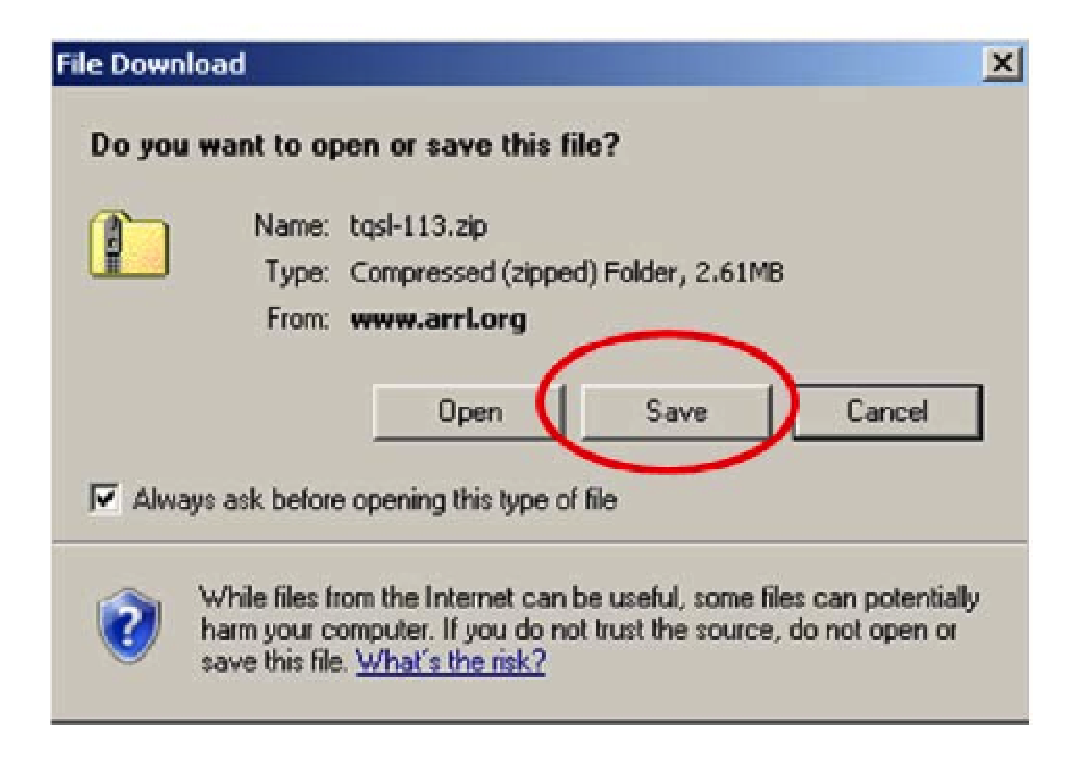
\includegraphics[width=0.58\textwidth]{win_save.eps}
			\caption{نافذة حفظ الملف}
			\label{fig:Save}
			\end{figure}
			عندما تظهر الشاشة السابقة قم بالضغط على حفظ \textenglish{Save} مع التأكد من مكان حفظ
		الملف كما هو موضح في الشكل\ref{fig:Save}.
		\item
			قم بالضغط مرتين على الملف \textenglish{TQSL} المضغوط و من ثم قم بالضغط مرتين على
		أيقونة \textenglish{TQSL-113} للبدأ في عملية تثبيت البرنامج.
\clearpage
			\begin{figure}[!hbtp]
			\centering
			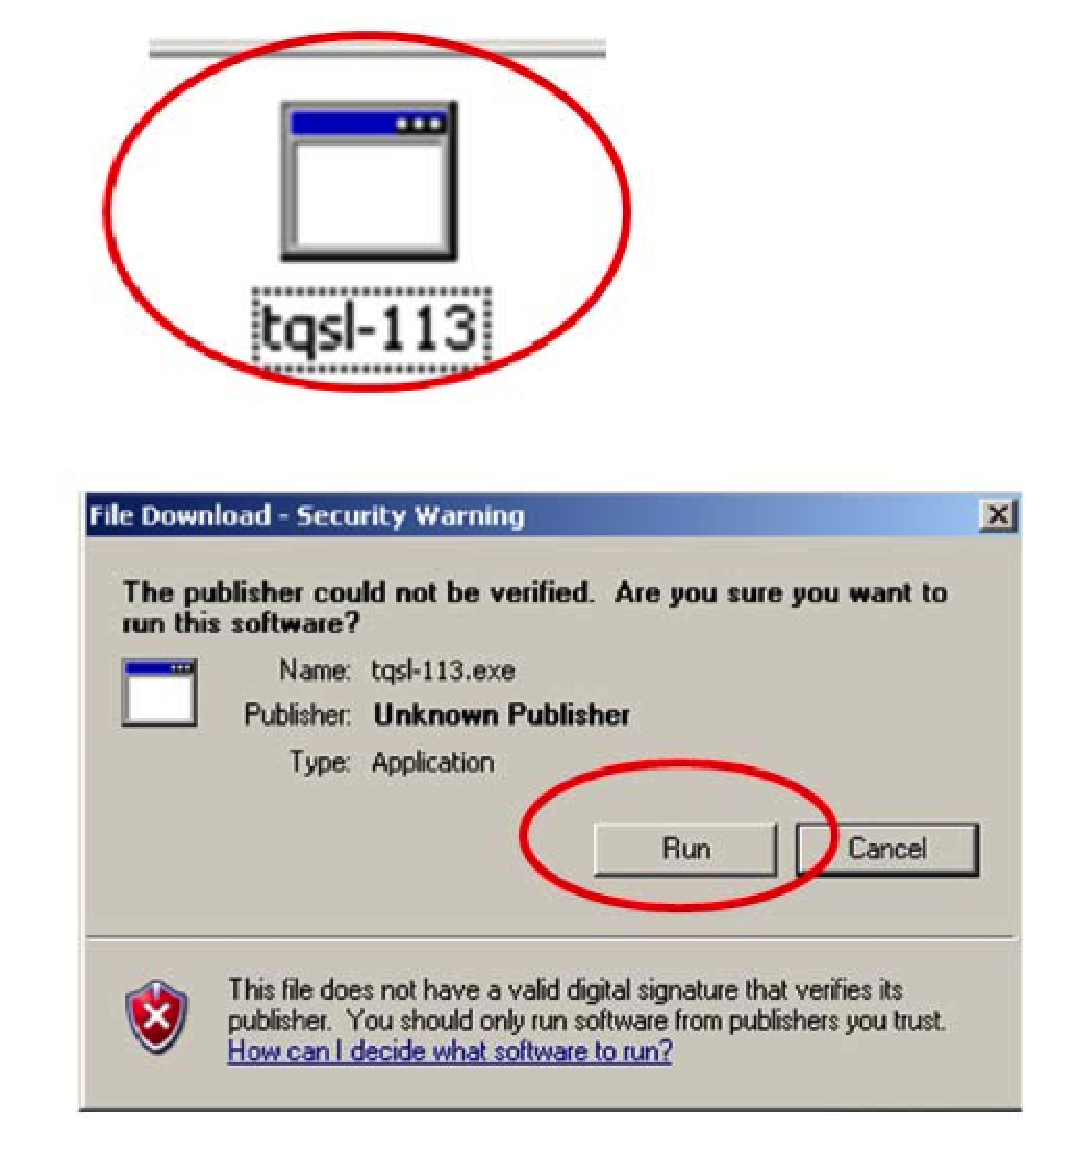
\includegraphics[width=0.58\textwidth]{tqsl113run.eps}
			\caption{ملف TQSL-113 ونافذة التشغيل}
			\label{fig:Run Window}
			\end{figure}
			\begin{itemize}
				\item
					\emph{في حال طلب منك الويندوز الإذن بتشغيل البرنامج اضغط على تشغيل
			أو \textenglish{Run}} كما هو موضح في الشكل \ref{fig:Run Window}.
				\item
					\emph{مستخدمي نظام ويندوز 7 وويندوز فيستا قد يتوجب عليهم تشغيل
			برنامج التثبيت كمدراء نظام \textenglish{Administrators}}.
			\end{itemize}
\clearpage
		\item
			\begin{figure}[!hbtp]
			\centering
			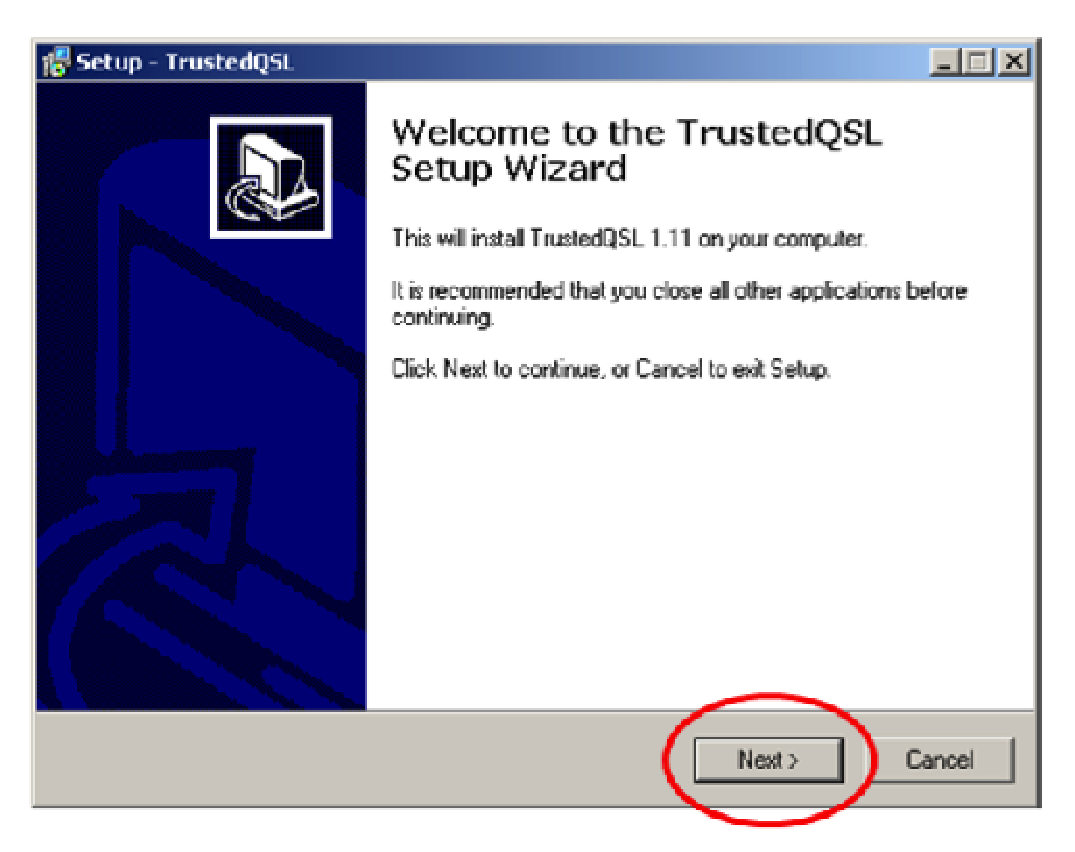
\includegraphics[width=0.58\textwidth]{installation-steps.eps}
			\caption{اضغط التالي Next لإتمام عملية التهيئة}
			\label{fig:Next}
			\end{figure}
			اضغط التالي \textenglish{Next} لإتمام عملية التثبيت ودع النظام يقوم بتثبيت البرنامج
		في المكان الإفتراضي كما هو موضح في الشكل \ref{fig:Next}.
		\item
			عند اكتمال التثبيت ستتوفر لديك أيقونتان جديدتان على سطح المكتب وهي
		التي سنستخدمها لتشغيل البرنامج الخاص بشهادات إشارة النداء \textenglish{TQSL} و \textenglish{TQSL Certificates}كما هو موضح في الشكل \ref{fig:Desktop}.
		
			\begin{figure}[!hbtp]
			\centering
			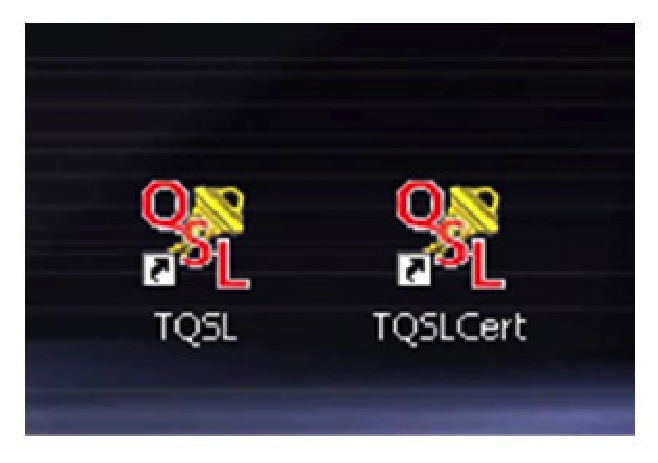
\includegraphics[width=0.3\textwidth]{desktop-icons.eps}
			\caption{أيقونتا البرنامج على سطح المكتب}
			\label{fig:Desktop}
			\end{figure}
		
	\end{enumerate}

أنت جاهز الآن للبدأ في الخطوة التالية (\ref{sec:2}) وهي طلب شهادة إشارة نداء.

% end of section
\vspace{24pt}
\begin{center}
	\color{slategray2}
{\Huge\hrulefill\hspace{0.2cm} \floweroneright\floweroneleft \hspace{0.2cm} \hrulefill}
\end{center}
\newpage

\section{الخطوة الثانية - طلب شهادة إشارة النداء}\label{sec:2}

طلب شهادة إشارة النداء عملية بسيطة تبدأ بإدخال بعض المعلومات الأساسية
عنك وحفظ الملف الذي ستقوم بإرساله إلى \textenglish{LoTW}.

\vspace{18pt}
\begin{center}
	\color{slategray2}
{\Huge \decoone}
\end{center}

\subsection{تفاصيل طلب شهادة إشارة النداء}

\textenglish{Logbook of the World} يعتمد على طريقة تشفير المفتاح الخاص والعام \textenglish{Public
key/Private key}. ولهذا فإن برنامج \textenglish{TrustedQSL} الذي قمت بتنزيله وتثبيته
على جهاز الكمبيوتر يحتوى على برنامجين أساسين - \textenglish{TrustedQSL}(\textenglish{TQSL}) وبرنامج
\textenglish{Trusted QSL Certificates (TQSL Cert)}. علماً أن جميع شهادات النداء تتم
إدارتها من خلال برنامج \textenglish{(TQSL Cert)}.  

ملف طلب شهادة إشارة النداء \textenglish{TQ5} يتم إرساله إلى \textenglish{\footnote{إتحاد نواب الراديو الأمريكي \textenglish{American Radio Relay League}}ARRL} ويتم الرد عليه بملف \textenglish{TQ6}. وعند تحميل ملف الـ \textenglish{TQ6} في برنامج \textenglish{TQSL Cert} سيتم إظهار شريطة ذهبية بجانب إشارة النداء والتي ستمكنك من استخدام الشهادة لختم دفتر السجلات إلكترونياً فيما بعد.

مَلَفَّي \textenglish{TQ5} و \textenglish{TQ6} يَحوِيانِ أختاماَ رقمية يجب مطابقتهما تماما مثل قطعتي
التذكرة المقطوعة. وأي طلبات شهادات إشارات النداء السابقة يتم تصفيرها عند
طلب شهادة إشارة نداء جديدة ولذلك لا تَقُم بحذف أو تعديل أي ملف بعد عمل طلب
شهادة إشارة نداء. ولوجوب ملائمة الطلب مع الرد فإن هذه العملية تتطلب إتمام ذلك من نفس جهاز الكمبيوتر. بعد حصولك على شهادة إشارة النداء كاملة يمكنك نقلها إلى أي جهاز كمبيوتر آخر باتباع الخطوات الموجودة في 
\href{http://www.arrl.org/advanced-lotw}{الدروس المتقدمة}.

طلب شهادة إشارة النداء ليس بعملية معقدة إطلاقاً. كل ما هو مطلوب إدخال بعض
المعلومات الأساسية عنك وعن إشارة ندائك ومن ثم حفظ ملف (ملف \textenglish{TQ5}) و
إرساله إلى دفتر سجلات العالم \textenglish{LoTW}.
\\

سنقوم الآن بتتبع الخطوات المطلوبة لطلب شهادة إشارة نداء خاصة بإشارة
ندائك الحالية. 
\\


\begin{enumerate}
	\item
		بعد تثبيتك لبرنامج \textenglish{Trusted QSL} ستجد أيقونتين على سطح المكتب:
  \clearpage
	\item
		\begin{figure}[!hbtp]
		\centering
		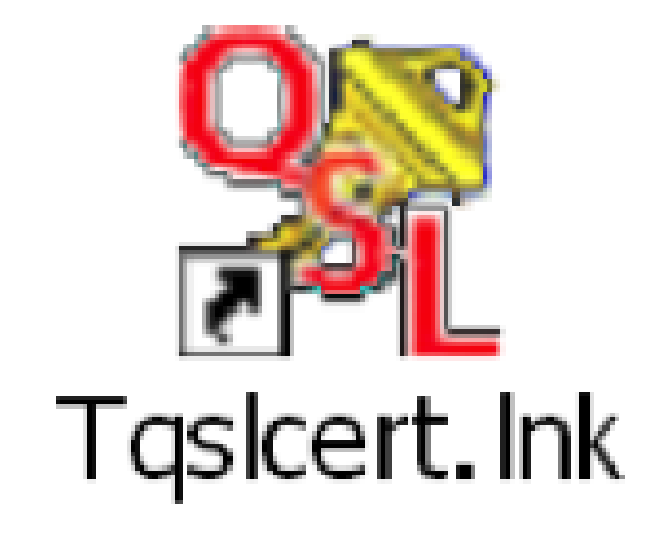
\includegraphics[width=0.1\textwidth]{tqslcert.eps}
		\caption{أيقونة البرنامج على سطح المكتب}
		\label{fig:Desktop2}
		\end{figure}
	  قم بفتح البرنامج \textenglish{TQSL Cert} بالنقر عليه مَرّتين كما هو موضح في الشكل \ref{fig:Desktop2}.
	\item
		عند فتح برنامج \textenglish{TQSL Cert} لأول مرة ستظهر رسالة بعدم وجود أي شهادة إشارة نداء لديك ويسألك إن كنت ترغب في طلب واحدة، قم باختيار \textenglish{Yes}.
	\item
		\begin{figure}[!hbtp]
		\centering
		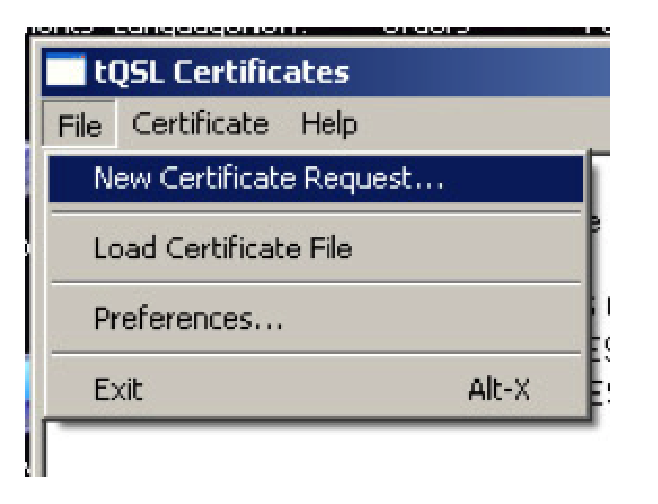
\includegraphics[width=0.4\textwidth]{newcsr.eps}
		\caption{طلب شهادة إشارة نداء جديدة}
		\label{fig:New CSR}
		\end{figure}
		
		في حال قيامك بالضغط على No بالخطأ في الرسالة السابقة؛ لا تفزع، يمكنك طلب ذلك من
		خلال اختيار \textenglish{File \textbar  New Certificate Request\ldots}  أي اضغط على
كلمة \textenglish{File} و من ثم اختر أول خيار وهو \textenglish{New Certificate Request} كما هو موضح في الشكل \ref{fig:New CSR}.
  \clearpage  
	\item
		\begin{figure}[!hbtp]
		\centering
		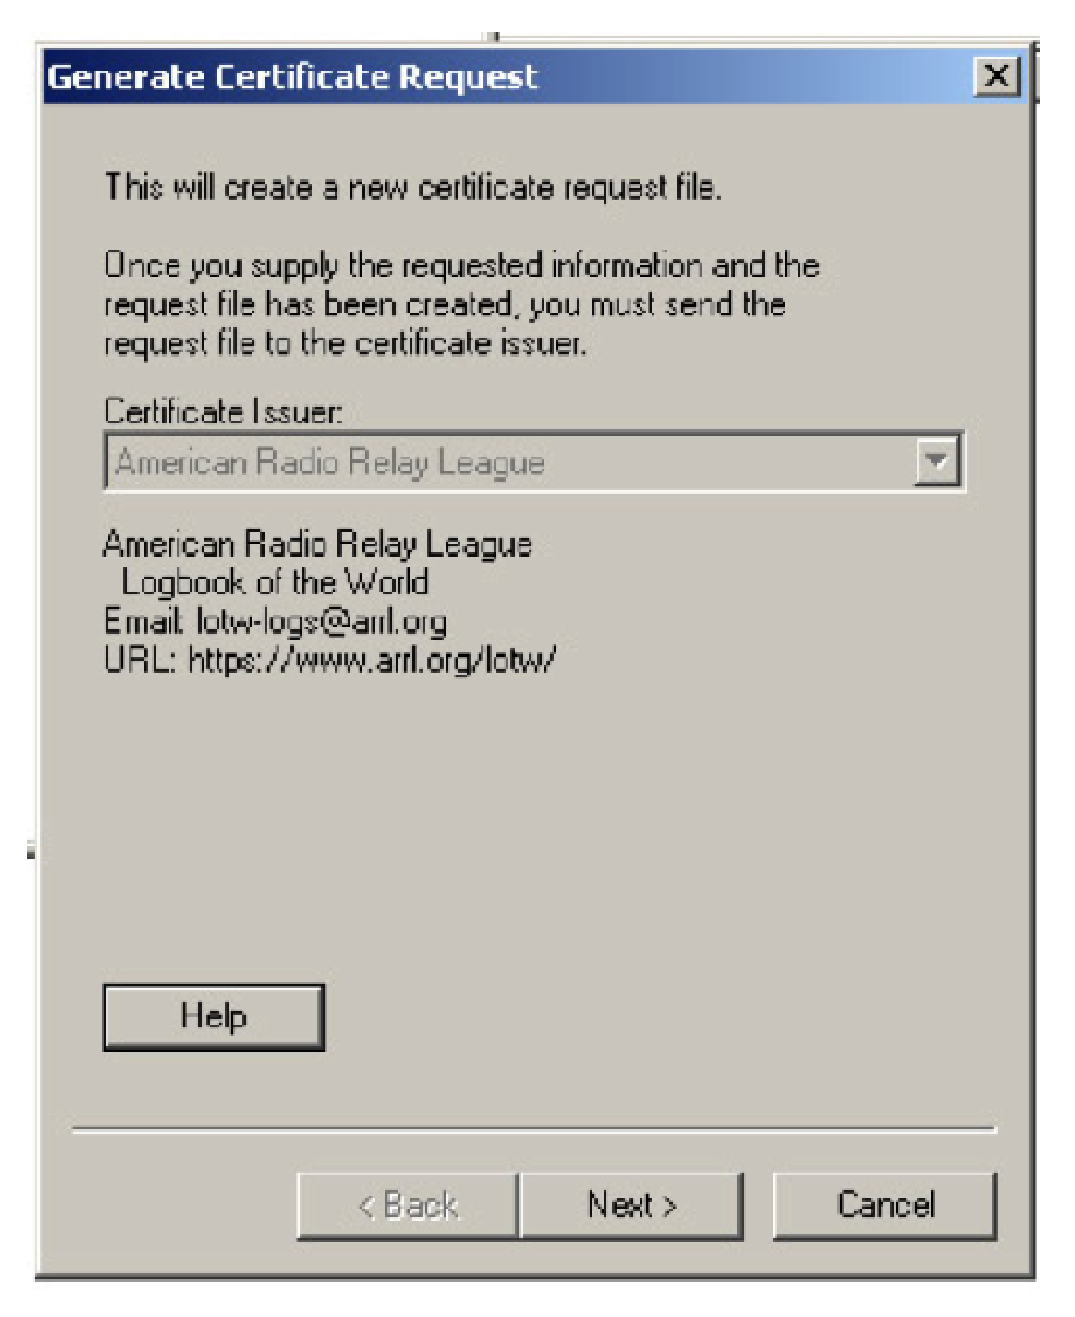
\includegraphics[width=0.4\textwidth]{generatecsr.eps}
		\caption{نافذة توضيحية فقط}
		\label{fig:ARRL Issuer}
		\end{figure}
		  أول نافذة تظهر هي رسالة توضيحية وتبين أن \textenglish{ARRL} هي صاحبة الحق في منحك شهادة
		  إشارة النداء. لا تتطلب هذه النافذة منك فعل أي شيء سوى الضغط على \textenglish{Next} كما هو موضح في الشكل \ref{fig:ARRL Issuer}.
	\item
		\begin{figure}[!hbtp]
		\centering
		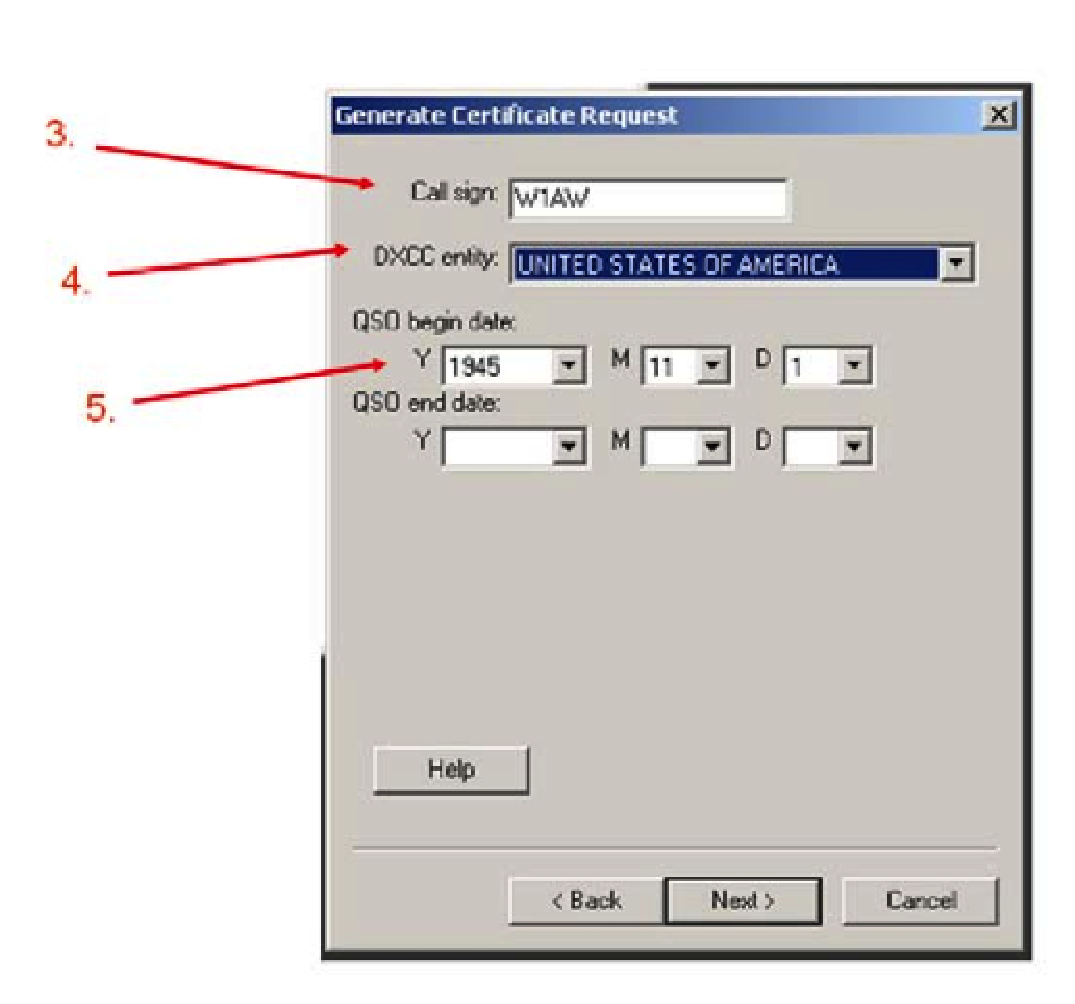
\includegraphics[width=0.53\textwidth]{callsign.eps}
		\caption{أدخل إشارة النداء بدون أي لَوَاحِق}
		\label{fig:Callsign}
		\end{figure}
		  أدخل الآن إشارة النداء الحالية الخاصة بك بدون أي لَوَاحق كما هو موضح في الشكل \ref{fig:Callsign}.
	\item 
		استخدم القائمة المُنسَدِلة لاختيار مكان وجودك والذي يتماشى مع إشارة ندائك ومن أين تقوم بالإتصال. أما إن كنت تحمل إشارة نداء \textenglish{KH6} أو \textenglish{KL7} و

		\begin{itemize}
			
			\item
				    عنوانك في الـ \textenglish{FCC}\footnote{\textenglish{FCC}: هي هيئة الإتصالات الفدرالية في أمريكا.} كان ولاية هاواي أو ألاسكا فإن الـ \textenglish{DXCC entity}\footnote{\textenglish{DXCC entity}: تعني كيانك أو موقعك الجغرافي حسب تقسيم \textenglish{DXCC} وهي اختصار لـ \textenglish{DX Century Club} أي نادي القرن للمحطات البعيدة.} الخاص بك سيكون هاواي أو ألاسكا.
			\item
				لو كان عنوانك في الـ \textenglish{FCC} هو إحدى الولايات الأمريكية فإن الـ \textenglish{DXCC entity} الخاص بك سيكون الولايات المتحدة الأمريكية.
		\end{itemize}

			\item
			 تاريخ الإتصالات \textenglish{QSO Date Range} سيقوم بتحديد الإتصالات الموجودة في دفتر السجلات الخاص بك والتي يمكن رفعها إلى موقع دفتر سجلات العالم \textenglish{Loogbook of The World}.
			\\
			من المهم التأكد من إدخال بيانات صحيحة إذ لن تتمكن من تعديل نطاق تاريخ
			الإتصالات \textenglish{QSO date range} بعد صدور شهادة إشارة النداء.

			\item
				  تاريخ بداية الإتصالات \textenglish{QSO Begin Date} يجب أن يكون تاريخ حصولك على إشارة النداء. وفي حال عدم تأكدك من التاريخ بالضبط يمكنك اختيار أول تاريخ إتصال مدون في دفتر سجلاتك الخاص بإشارة النداء هذه.
				\begin{itemize}
					\item
						لاتستخدم تاريخ اليوم!
					\item
						لا يفترض أن يكون هذا التاريخ تاريخ حصولك على أول إشارة نداء إن كانت لك إشارة نداء سابقة!
					\item
						لا تستخدم تاريخ ميلادك!
				\clearpage
					\item
						\begin{figure}[!hbtp]
						\centering
						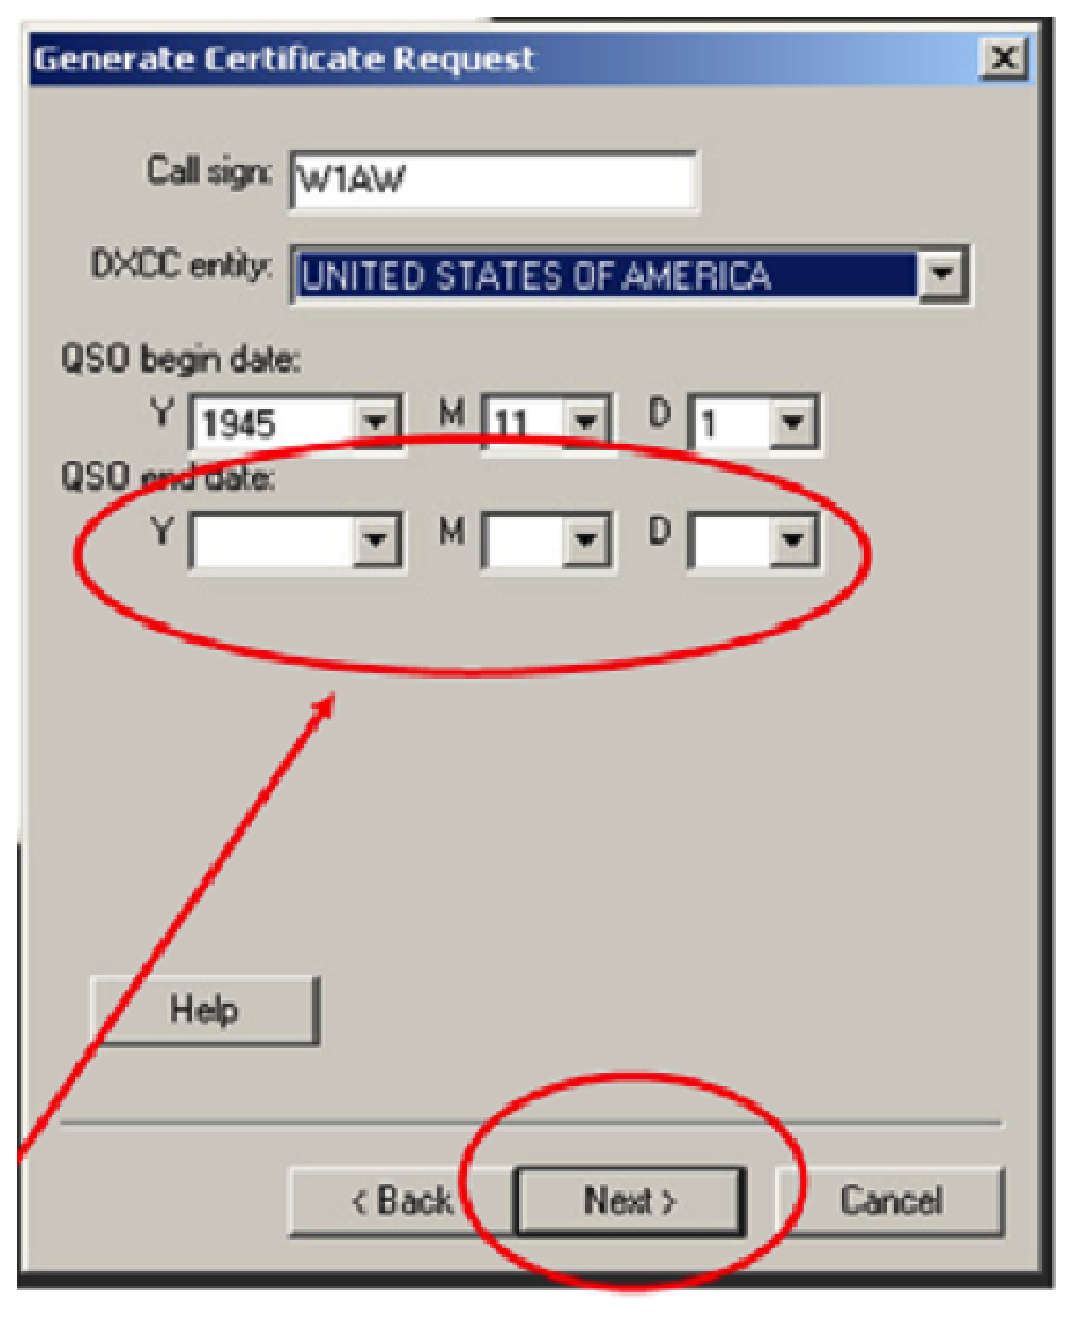
\includegraphics[width=0.4\textwidth]{csrenddate.eps}
						\caption{يجب أن يكون هذا الحقل فارغا}
						\label{fig:CSR End Date}
						\end{figure}
						لا تستخدم تاريخ إنتهاء الإتصالات \textenglish{QSO End Date} لإشارة ندائك حيث
						أن ذلك سيحد الإتصالات إلى ذلك التاريخ فقط كما هو موضح في الشكل \ref{fig:CSR End Date}.

				\end{itemize}
			\item
				\begin{figure}[!hbtp]
				\centering
				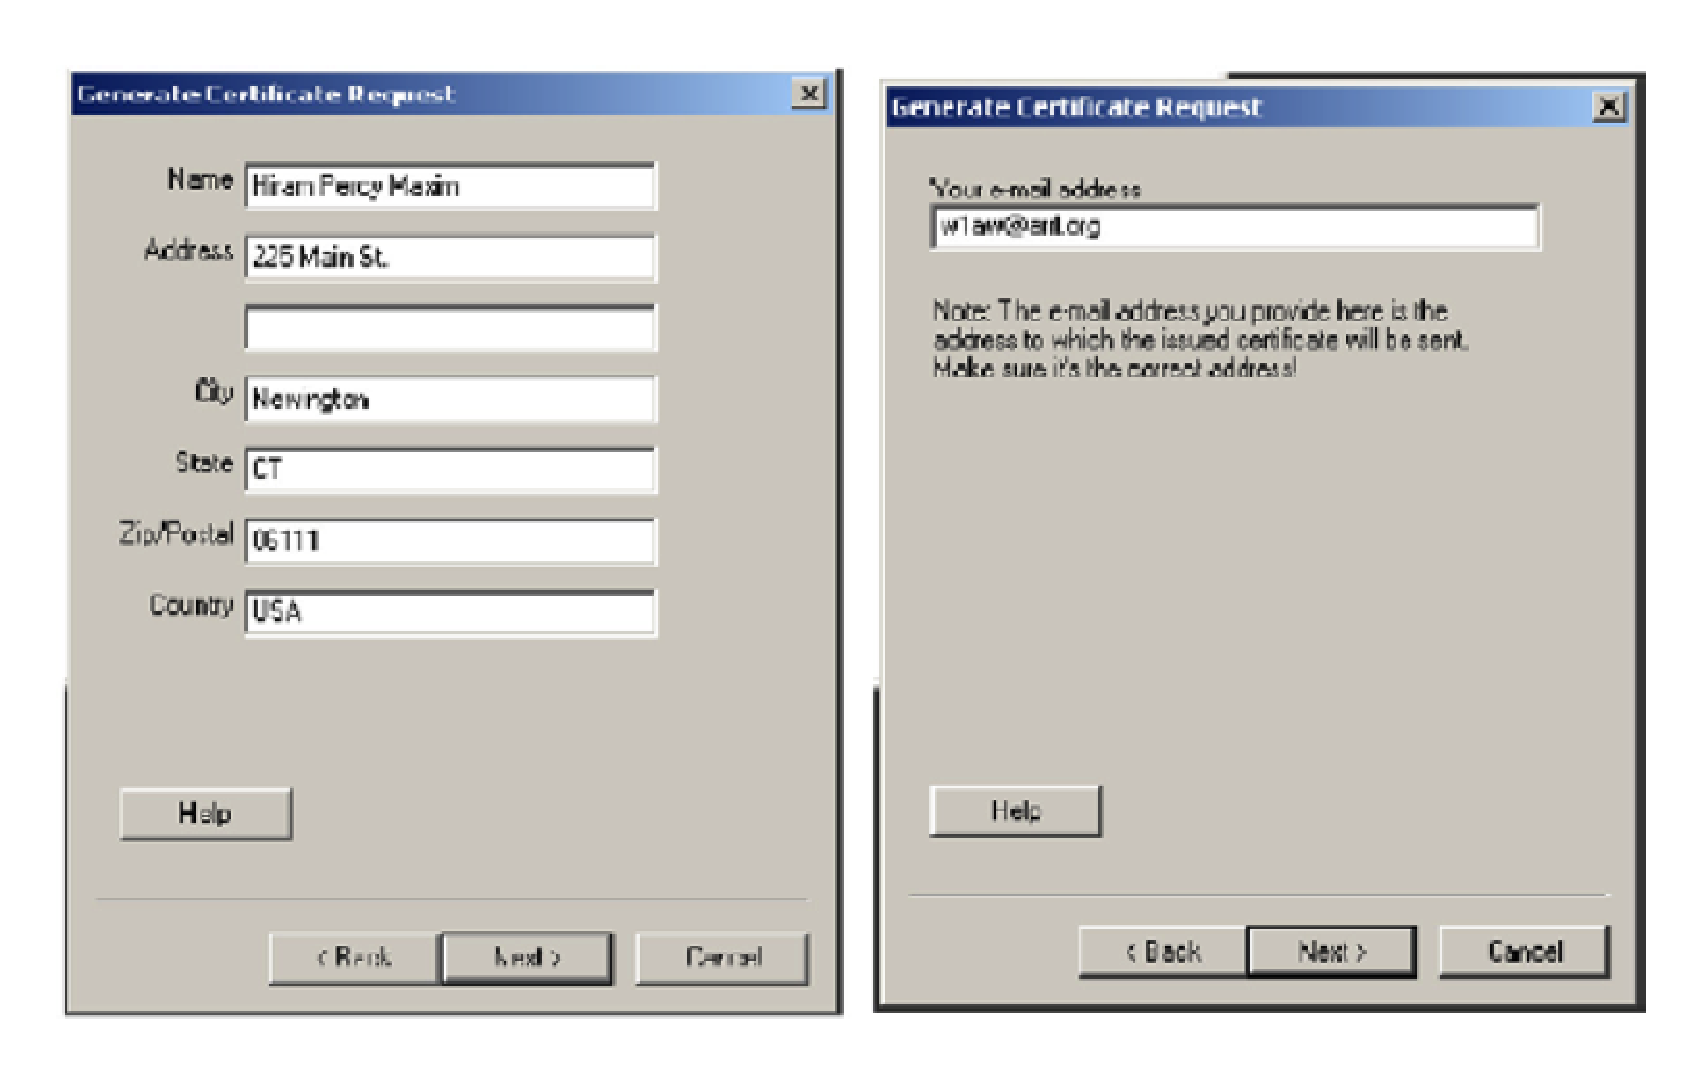
\includegraphics[width=0.84\textwidth]{csrname.eps}
				\caption{أدخل اسمك وعنوانك}
				\label{fig:CSR Name}
				\end{figure}
				أدخل اسمك وعنوانك ولسكان الولايات المتحدة الأمريكية يجب أن يتطابق العنوان مع العنوان المدخل في الـ \textenglish{FCC} ثم اضغط \textenglish{Next} كما هو موضح في الشكل \ref{fig:CSR Name}.

			\item
				أدخل عنوان بريدك الإلكتروني.
				\begin{itemize}
					\item
						تأكد من أن مزود خدمة البريد الإلكتروني يسمح لك باستقبال المرفقات. إذ أنك ستستقبل ملف شهادة إشارة النداء \textenglish{TQ6} واسم المستخدم وكلمة المرور على البريد الإلكتروني.
				\end{itemize}
				

\paragraph{هذه الخطوة اختيارية:}
يفضل استخدامك لكلمة مرور خصوصا إذا كان الجهاز المستخدم جهاز عام وليس خاص
بك أو لو كنت تستخدم برنامج \textenglish{TQSL} على جهاز محمول. وفي حال استخدامك لكلمة
مرور الرجاء التأكد من كتابتها وحفظها في مكان آمن حتى لا تنساها. أما في
حال نسيانها فيؤسفنا إبلاغك بأن \textenglish{ARRL} لن تتمكن من مساعدتك في استرجاعها.
ولاستعادة ذلك يجب طلب شهادة إشارة نداء جديدة.

		\begin{figure}[!hbtp]
		\centering
		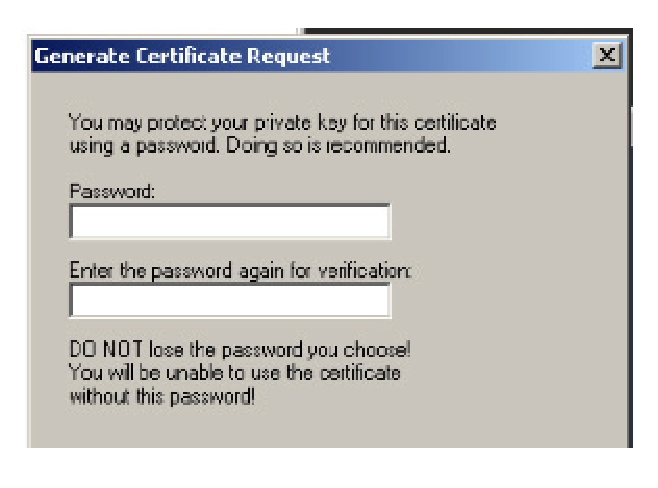
\includegraphics[width=0.5\textwidth]{generatecsrpassword.eps}
		\caption{أدخل كلمة المرور في حال أردت ذلك}
		\label{fig:Password}
		\end{figure}
			\item
			أدخل كلمة المرور إن أردت كما هو موضح في الشكل \ref{fig:Password}.
				\begin{itemize}
					\item
					يمكنك ترك هذا الحقل فارغا (ينصح بذلك للأجهزة الشخصية)

				\end{itemize}
			\item
			\clearpage
				\begin{figure}[!hbtp]
				\centering
				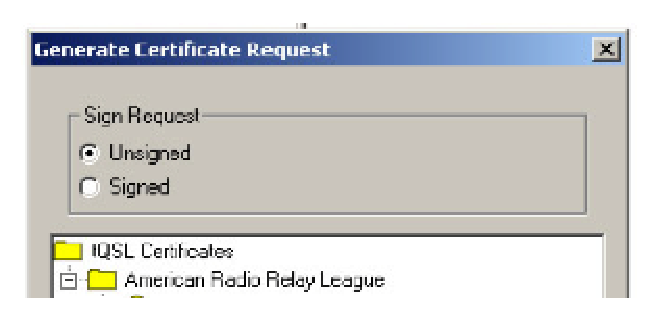
\includegraphics[width=0.5\textwidth]{unsigned.eps}
				\caption{تأكد من اختيار Unsigned}
				\label{fig:Unsigned}
				\end{figure}
			تأكد من أن طلبك لم يتم ختمه بعد \textenglish{Unsigned} كما هو موضح في الشكل \ref{fig:Unsigned}.
				\begin{itemize}
					\item
					سيكون غير مختوم \textenglish{Unsigned} هو الخيار الوحيد لك وذلك لأن هذه أول شهادة إشارة نداء لك.
				\end{itemize}
\end{enumerate}
		\begin{figure}[!hbtp]
		\centering
		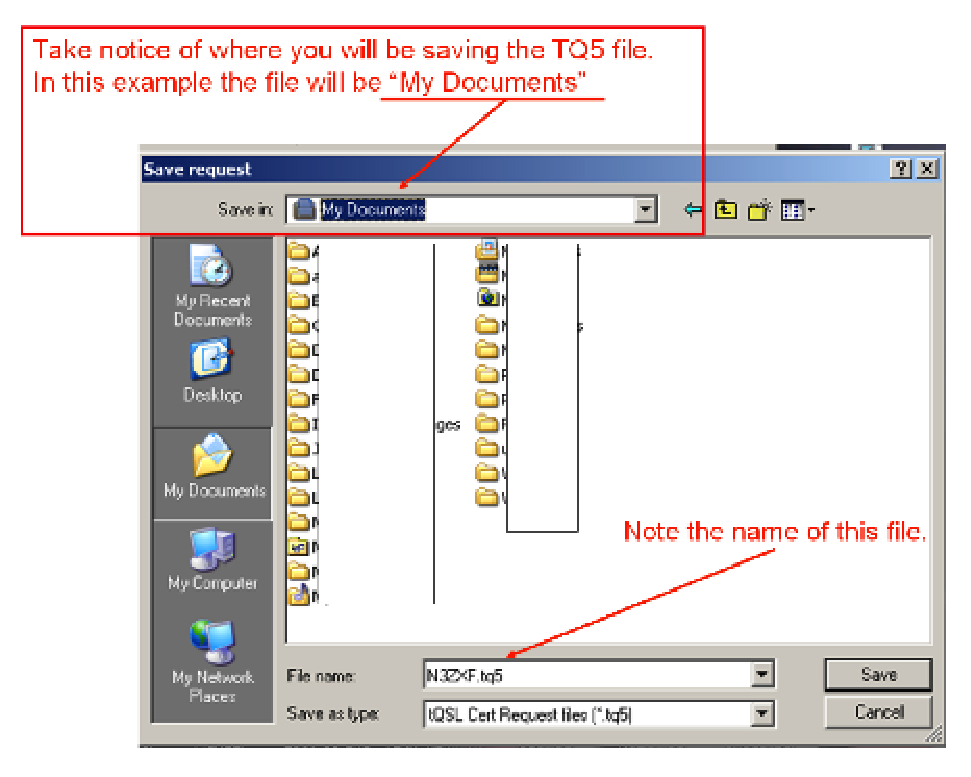
\includegraphics[width=0.8\textwidth]{filesaveloc.eps}
		\caption{تأكد من مكان حفظ الملف}
		\label{fig:FileSave}
		\end{figure}
تأكد من مكان حفظ الملف كما هو موضح في الشكل \ref{fig:FileSave} وستكون بهذا قد حفظت ملف \textenglish{TQ5} الذي يتوجب عليك
إرساله بعد قليل.

\newpage
				\begin{figure}[!hbtp]
				\centering
				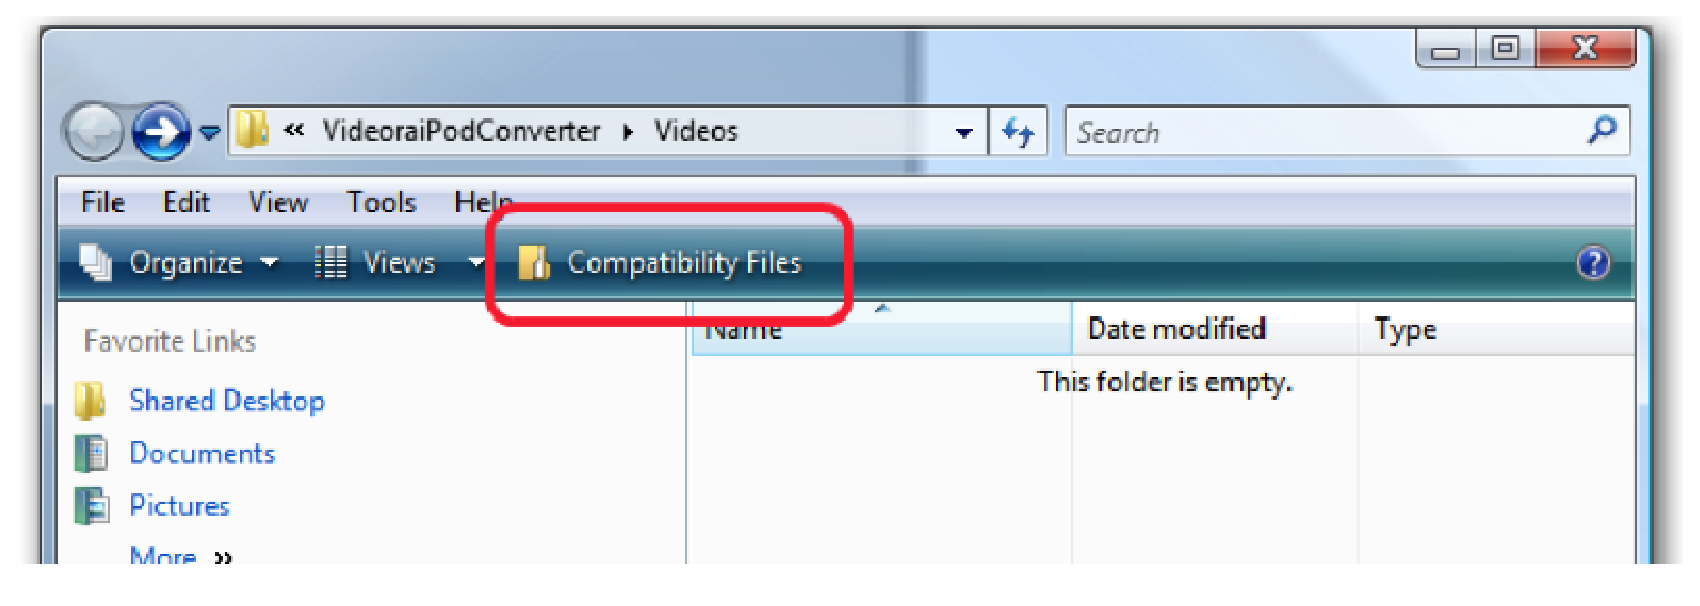
\includegraphics[width=0.9\textwidth]{compatbefore.eps}
				\caption{خاصية صلاحيات الملفات التوافقية}
				\label{fig:Compat}
				\end{figure}
\begin{quote}
\textbf{مستخدمي ويندوز فيستا:} يجب أن تكون مُفَعِّلا لخاصية \emph{صلاحيات الملفات التوافقية\footnote{خاصية الملفات التوافقية والتي تسمى \textenglish{Compatibility files}}} كما هو موضح في الشكل \ref{fig:Compat}.
إن كنت ترى هذا المجلد قم بالضغط عليه للسماح بتوافقية الملفات وإلّا فلن
تتمكن من رؤية ملف \textenglish{TQ5} الذي قمت بحفظه. بعد الضغط على مجلد صلاحيات الملفات التوافقية (\textenglish{Compatibility files}) سيتغير شكله إلى أيقونة (حرق) أو (\textenglish{Burn}) كما هو موضح أدناه في الشكل \ref{fig:CompatAft}.
\end{quote}

				\begin{figure}[!hbtp]
				\centering
				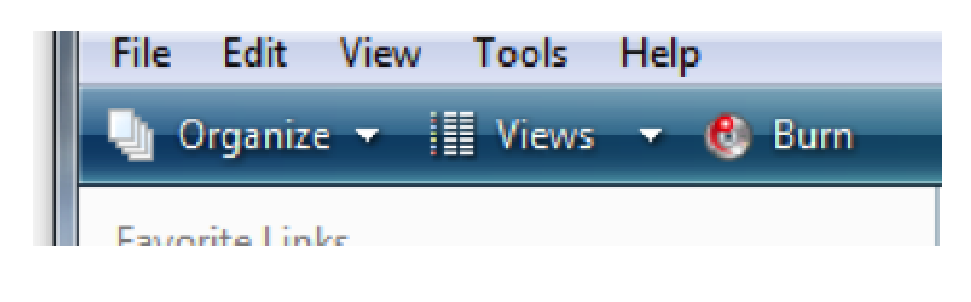
\includegraphics[width=0.6\textwidth]{compatafter.eps}
				\caption{خاصية صلاحيات الملفات التوافقية بعد تفعيلها}
				\label{fig:CompatAft}
				\end{figure}

\vspace{18pt}
\begin{center}
	\color{slategray2}
{\Huge \decoone}
\end{center}

			\clearpage
يجب أن تعلم بأن رفع الملف ليس تلقائياً. بل يتطلب ذلك أن تُكمل الخطوة التالية لرفع
ملف \textenglish{TQ5} الذي قُمت بحفظه قبل قليل من خلال موقع \textenglish{ARRL} أو إرسال الملف إلى
البريد الإلكتروني lotw-logs@arrl.org كما هو موضح في الشكل \ref{fig:Send}
\\
				\begin{figure}[!hbtp]
				\centering
				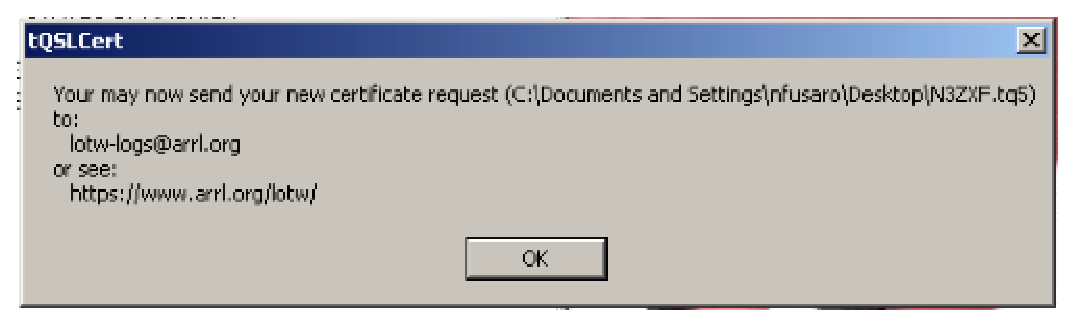
\includegraphics[width=0.6\textwidth]{csrsend.eps}
				\caption{يمكنك الآن إرسال أو رفع ملف الـ TQ5}
				\label{fig:Send}
				\end{figure}

عند إتمام العملية بشكل سليم ستظهر نافذة \textenglish{TQSL Cert} وبها دائرة حمراء
وبداخلها خط تماما مثل إشارة ممنوع الدخول بجانب إشارة ندائك وموقعك تماما كما هو موضح في الشكل \ref{fig:RedCircle}.
				\begin{figure}[!hbtp]
				\centering
				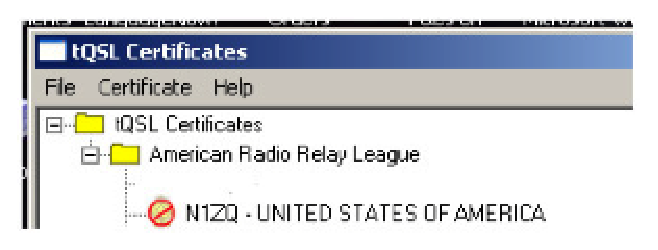
\includegraphics[width=0.6\textwidth]{redcircle.eps}
				\caption{شكل إشارة النداء وهي غير مختومة. لاحظ وجود الدائرة الحمراء}
				\label{fig:RedCircle}
				\end{figure}
\vfill
{\large\textbf{{\color{oucrimsonred}ومن المهم عدم حذف أو نقل أو إعادة تسمية ملف \textenglish{TQ5} ولا حذف الدائرة الحمراء!.}}}

\vspace{18pt}
\begin{center}
	\color{slategray2}
{\Huge \decoone}
\end{center}

\clearpage

\subsection{طرق رفع ملف طلب شهادة إشارة النداء (\textenglish{TQ5})}

\begin{enumerate}
		\item
			الذهاب إلى صفحة رفع الملفات في \textenglish{LoTW} وهي \href{https://p1k.arrl.org/lotw/upload}{\textenglish{https://p1k.arrl.org/lotw/upload}}.
		\item
			\begin{figure}[!hbtp]
			\centering
			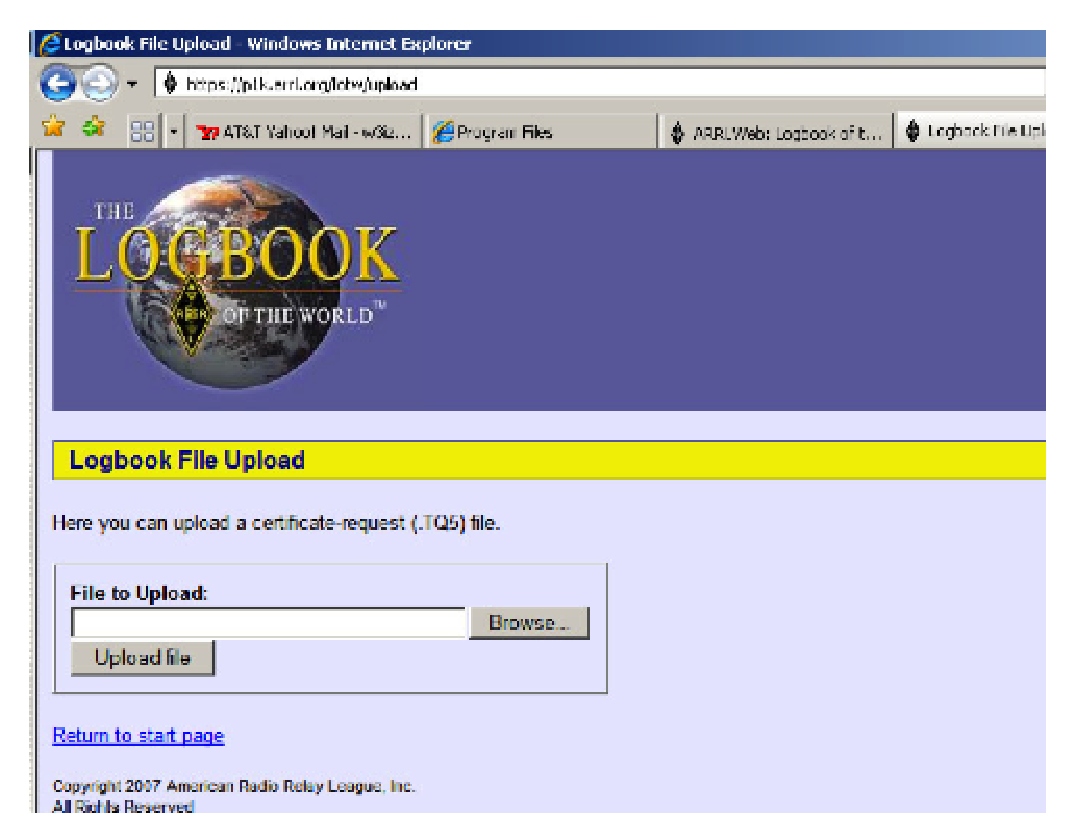
\includegraphics[width=0.7\textwidth]{LoTWUpload.eps}
			\caption{صفحة LoTW لرفع الملفات}
			\label{fig:LoTW}
			\end{figure}
			
			اضغط على تصفح (\textenglish{Browse}) لتحديد واختيار ملف الـ \textenglish{TQ5} من جهازك والذي قمت بحفظه في الخطوة السابقة كما هو موضح في الشكل \ref{fig:LoTW}.
			
		\item
			قم برفع الملف.
		\item
			يجب أن تنتظر وصول البطاقة البريدية عبر البريد.

			\begin{itemize}
					\item
						إن كنت تقوم بإرسال طلب شهادة إشارة نداء لإشارة نداء غير أمريكية فإنه يتوجب عليك توفير وإرسال صورة من رخصة الهواية والصادرة من بلدك و صورة من إثبات هويتك والتي يظهر فيها اسمك مثل رخصة قيادة السيارة مثلا. تفضل بزيارة \href{https://www.arrl.org/lotw/docreq}{\textenglish{https://www.arrl.org/lotw/docreq}} لمزيد من التفاصيل.
			\end{itemize}
\end{enumerate}

{\large\textbf{{\color{oucrimsonred}البطاقات البريدية والأوراق الثبوتية مطلوبة فقط للتسجيل لأول مرة لفتح الحساب و لا حاجة لها بعد ذلك.}}}

% end of section
\vspace{20pt}
\begin{center}
	\color{slategray2}
{\Huge\hrulefill\hspace{0.2cm} \floweroneright\floweroneleft \hspace{0.2cm} \hrulefill}
\end{center}
\newpage


\section{الخطوة الثالثة - تصديق موقعك (داخل أمريكا)}
يتم تصديق العنوان لهواة الراديو في أمريكا من خلال إرسال بطاقة بريدية إلى
عنوانك المسجل في قاعدة بيانات \textenglish{FCC}. يجب عليك تحديث العنوان إن كان غير صحيح أو بحاجة إلى تحديث من خلال موقع  \href{http://wireless.fcc.gov/uls}{\textenglish{FCC ULS}\footnote{\textenglish{FCC ULS}: هي اختصار لـ \textenglish{FCC Universal Licensing System} أي نظام الرخص العالمي لهيئة الإتصالات الفدرالية بأمريكا.}} بعد ذلك يجب عليك زيارة موقع \textenglish{LoTW} وإدخال الرمز المكون من 8 خانات والموجود في
البطاقة البريدية. ثم سيتم إرسال ملف \textenglish{TQ6} من خلال البريد الإلكتروني الخاص بك.

% end of section
\vspace{24pt}
\begin{center}
	\color{slategray2}
{\Huge\hrulefill\hspace{0.2cm} \floweroneright\floweroneleft \hspace{0.2cm} \hrulefill}
\end{center}
\vspace{24pt}
\section{الخطوة الثالثة - تصديق موقعك (خارج أمريكا)}

يجب إرسال صورة من رخصة هاوي اللاسلكي و صورة من إثبات الهوية مثل رخصة
القيادة أو جواز السفر لتصديق موقع أي محطة خارج أمريكا إلى العنوان
التالي:

\begin{flushleft}
	\begin{verbatim}
		ARRL LoTW Administrator
		225 Main St.
		Newington, CT 06111
	\end{verbatim}
\end{flushleft}

الرجاء عدم إرسال أي وثيقة إلكترونيا. يجب أن يكون الظرف مُعَنوَناً ويحمل
عنوانك الحقيقي. بإمكانك اتباع الرابط التالي لمعرفة كافة الأوراق الثبوتية التي يمكن
قبولها.\par
\href{https://p1k.arrl.org/lotw/docreq}{https://p1k.arrl.org/lotw/docreq}

\vspace{18pt}
\begin{center}
	\color{slategray2}
{\Huge \decoone}
\end{center}

\subsection{تفاصيل تصديق موقعك}

أي محطة غير أمريكية تَطلُب الحصول على شهادة إشارة النداء يجب أن تقوم
بتوفير صورة من رخصة مزاولة الهواية (رخصة هواة اللاسلكي) وكذلك صورة من أي
وثيقة رسمية مثل رخصة القيادة أو جواز السفر والتي يظهر فيها اسم مُقدم
الطلب وصورته وذلك فقط لأول مرة يُطلب فيها إنشاء حساب في دفتر سجلات العالم
\textenglish{Loogbook of the World}. علما أنه سيتم اتخاذ الإجراءات اللازمة للتأكد من
إتلاف هذه الوثائق فور التأكد من هوية مُقدم الطلب بشكل سليم. كل هذه
الوثائق يجب إرسالها بواسطة البريد إلى مقر إدارة \textenglish{ARRL} كما هو موضح في
العنوان التالي. \textbf{لن يتم قبول أي رسائل إلكترونية في هذا الخصوص} لأن استخدام
البريد لتوثيق إشارة نداء مُقدم الطلب يساعد في حماية إشارة ندائك من سوء
الاستخدام ويساعدنا في التحقق من طلبات المستخدمين.

يجب إرسال جميع الوثائق المطلوبة عبر البريد إلى العنوان التالي:
\begin{flushleft}
	\begin{verbatim}
	Logbook Administration
	ARRL
	225 Main Street
	Newington, CT 06111
	USA
	\end{verbatim}
\end{flushleft}

يمكن طلب شهادة إشارة نداء أخرى لإشارة نداء جديدة أو سابقة لأي مُشغل محطة
قام بإصدار شهادة إشارة نداء مِن قَبْل وذلك دون الحاجة لطلب أوراق ثبوتية
جديدة ولكن لكل طلب شهادة جديدة يجب تقديم ما يُثبت أَحَقية استخدام إشارة
النداء تِلك إلا في الحالات التالية:

	\begin{itemize}
		\item
			العمل تحت اتفاقية \textenglish{CEPT} أو \textenglish{IARP} أو
		\item
			العمل تحت اتفاقية بين دولتين أو أكثر بحيث لا يَتطلب ذلك الحصول على رخصة أو ترخيص تشغيل إضافي.
	\end{itemize}

اتفاقية التشغيل المتبادَلة بين دولتين خارج اتفاقية \textenglish{CEPT} لا تُلغي الحاجة
إلى إثباتات \textenglish{LoTW} المطلوبة. وفي حال عدم تَوَفُّر الوثائق أو ما يُثبِت أحقية
استخدامك لإشارة نداء سابقة فإنه يُمْكِنك التواصل معنا لإرشادك إلى الخطوات
المطلوبة ولا حاجة لأوراق ثبوتية الهوية إن كان طلب شهادة إشارة النداء
الجديد سيتم ختمه بشهادة موجودة مسبقة على نفس الجهاز.

في حال طُلِب منك توفير أوراق ثبوتية الهوية مثل صورة من رخصة القيادة أو
صورة من جواز السفر رغم وجود شهادة مُصدقة لديك مسبقا فإنه في هذه الحالة
فقط يمكنك إرسال صورة من تلك الوثائق عبر البريد الإلكتروني إلى العنوان
\href{mailto:LoTW-help@arrl.org}{LoTW-help@arrl.org} تذكر أنه يمكنك إرسال ذلك فقط لطلبات الشهادات
الإضافية وليس لطلبك الأساسي.


% end of section
\vspace{24pt}
\begin{center}
	\color{slategray2}
{\Huge\hrulefill\hspace{0.2cm} \floweroneright\floweroneleft \hspace{0.2cm} \hrulefill}
\end{center}
\newpage

\section{الخطوة الرابعة - تحميل ملف شهادة إشارة النداء (الملف \textenglish{TQ6})}

في هذه المرحلة يجب أن تكون قد استلمت بريدا إلكترونيا من \textenglish{LoTW} وبه ملف الـ
\textenglish{TQ6} الخاص بك. رسالة البريد الإلكتروني هذه ستحتوي أيضا على اسم المستخدم
(إشارة نِدائِك) وكلمة السر الخاصة للدخول إلى صفحة \textenglish{LoTW} الخاصة بك وستجد هذه
البيانات في أسفل نص الرسالة.

سترشدك هذه التعليمات إلى كيفية تحميل ملف الـ \textenglish{TQ6} وأهم من ذلك كيف ستقوم
بحفظ شهادة إشارة النداء. إذ أن ملف الـ \textenglish{TQ6} بحد ذاته لا يعتبر مَلف
شهادة النداء ولذلك يجب التأكد من اتِّباع التعليمات لتحميل وحفظ تلك
الشهادة.

\vspace{18pt}
\begin{center}
	\color{slategray2}
{\Huge \decoone}
\end{center}

\subsection{تفاصيل تحميل ملف شهادة إشارة النداء}

\subsubsection{تحميل ملف الشهادة}

	\begin{enumerate}
		\item
		\begin{figure}[!hbtp]
		\centering
		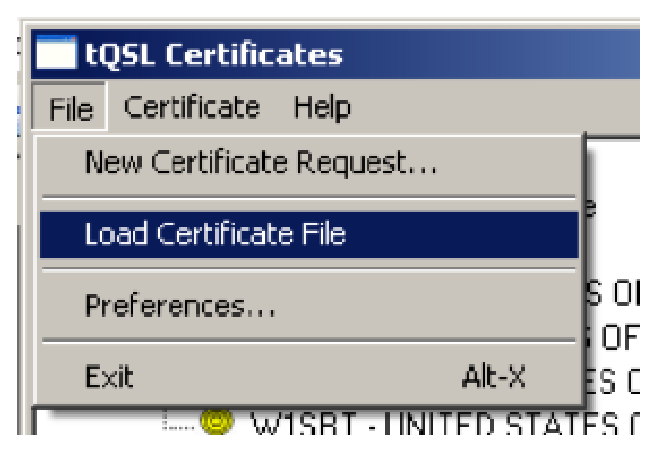
\includegraphics[width=0.4\textwidth]{loadcert.eps}
		\caption{تحميل ملف الشهادة TQ6 من برنامج \textenglish{TQSL Cert}}
		\label{fig:LoadTQ6}
		\end{figure}
			بإمكانك الضغط مرتين على الملف الذي استلمته عبر البريد الإلكتروني (ملف \textenglish{TQ6}) ومن ثم اضغط على نعم \textenglish{Yes} لفتحه حيث سيتم تحميله في البرنامج تلقائيا -- أو -- يمكنك حفظ الملف في المجلد \textenglish{LoTW} ومن ثم استخدام خاصية
		  استيراد الملف من تطبيق \textenglish{TQSL Cert} من خلال اختيار \textenglish{Load Certificate File}
		  من قائمة \textenglish{File} كما هو موضح في الشكل \ref{fig:LoadTQ6}.
\clearpage
		\item
		\begin{figure}[!hbtp]
		\centering
		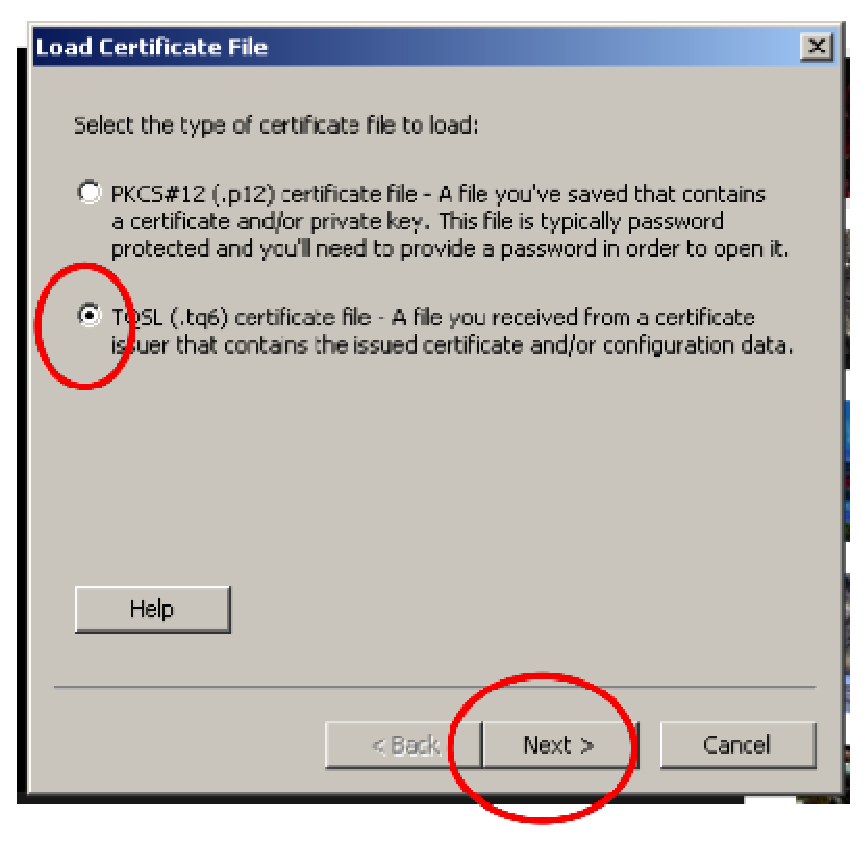
\includegraphics[width=0.5\textwidth]{tq6.eps}
		\caption{تأكد من اختيارك للخَيار الثاني TQ6}
		\label{fig:selectTypeTQ6}
		\end{figure}
			تأكد من اختيارك للملف \textenglish{TQ6} ومن ثم اختر التالي \textenglish{Next} كما هو موضح في الشكل \ref{fig:selectTypeTQ6}.
		\item	
		\begin{figure}[!hbtp]
		\centering
		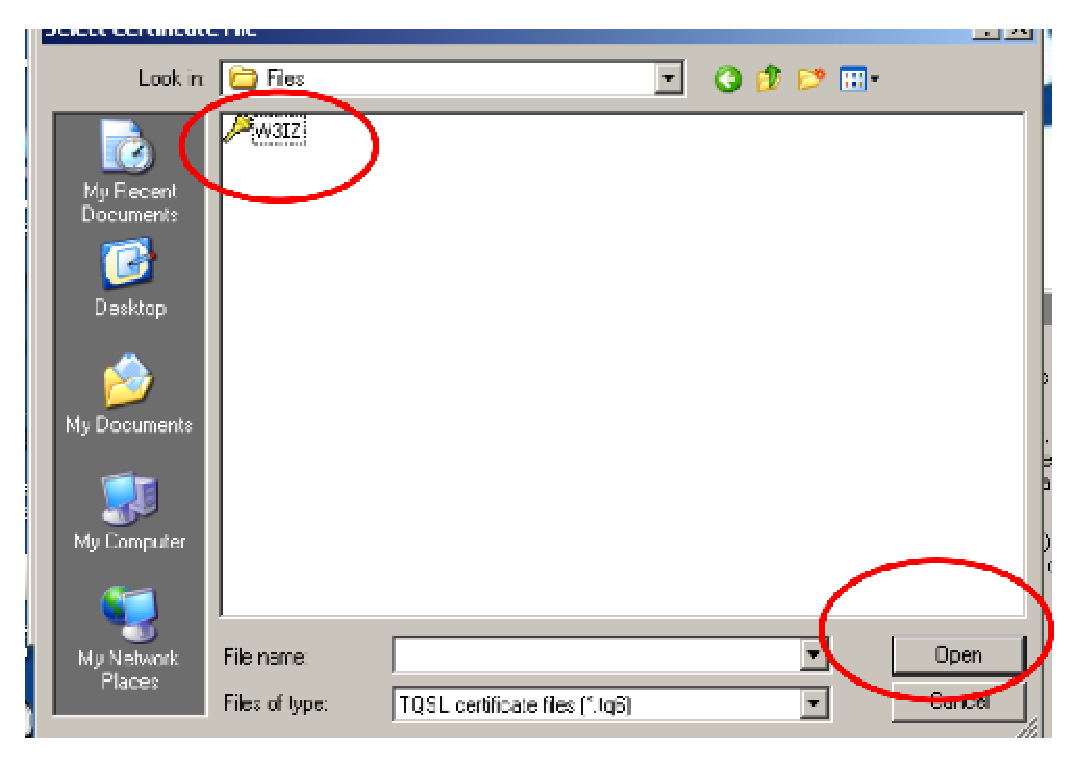
\includegraphics[width=0.6\textwidth]{selectfiletoload.eps}
		\caption{اختر الملف الصحيح لتحميله في البرنامج}
		\label{fig:SelectTQ6File}
		\end{figure}
			  اختر ملف الـ \textenglish{TQ6} والذي قمت بحفظه من مُرفقات البريد الإلكتروني كما هو موضح في الشكل \ref{fig:SelectTQ6File}.
\clearpage
		\item
		\begin{figure}[!hbtp]
		\centering
		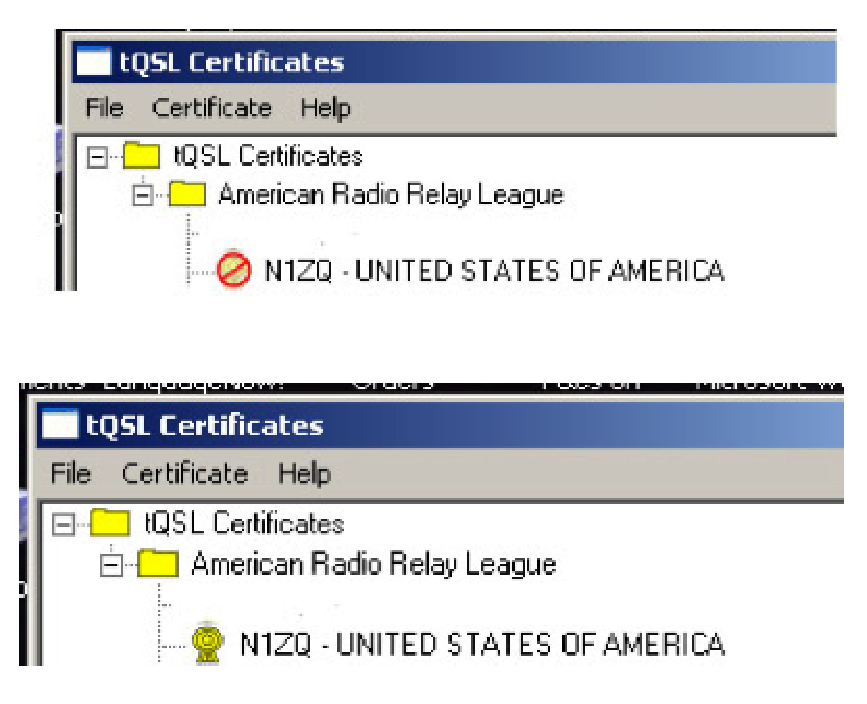
\includegraphics[width=0.6\textwidth]{unsignedsigned.eps}
		\caption{تغيير الدائرة الحمراء بشريطة ذهبية}
		\label{fig:UnSignedSigned}
		\end{figure}
			  ستتبدل الدائرة الحمراء بشريطة ذهبية عند تحميل الملف بشكل سليم كما هو موضح في الشكل \ref{fig:UnSignedSigned}.

\vspace{18pt}
\begin{center}
	\color{slategray2}
{\Huge \decoone}
\end{center}

\subsubsection{حفظ الشهادة}
		\begin{figure}[!hbtp]
		\centering
		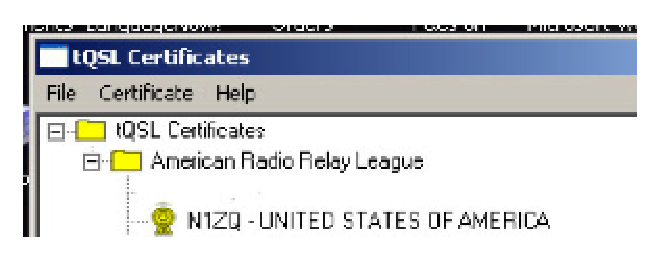
\includegraphics[width=0.6\textwidth]{signed.eps}
		\caption{الشهادة بعد استيراد ملف \textenglish{TQ6}}
		\label{fig:SignedTQ6}
		\end{figure}
يجب أن تكون الدائرة الحمراء في برنامج \textenglish{TQSL Cert} قد تم استبدالها بالشريطة
الذهبية قبل الخوض في الخطوة التالية تماما كما هو موضح في الشكل \ref{fig:SignedTQ6}. إذ يجب عليك الآن حفظ الشهادة كاملة
كملف من نوع \textenglish{p12} لأي قرص حفظ خارجي أو قرص مدمج \textenglish{CD} أو فلاش \textenglish{USB}. ذلك لأنه
في حال تم تعطل جهازك الحالي لأي سبب من الأسباب فإنه يمكنك إعادة استيراد
الشهادة من خلال هذا الملف \textenglish{p12} في برنامج \textenglish{TQSL Cert}.

لقد قام المَلَفّان \textenglish{TQ5} و \textenglish{TQ6} بدورهما الآن ولسنا بحاجة لحفظ أي منهما في مكان
ما. إلا أنه يجب المحافظة على الملف p12 لتتمكن من استيراده لاحقا إذا لزم
الأمر.


		\item
			  قم بفتح برنامج \textenglish{TQSL Cert} من خلال الضغط على أيقونته من سطح المكتب \ref{fig:Desktop2}.
		\item
		\begin{figure}[!hbtp]
		\centering
		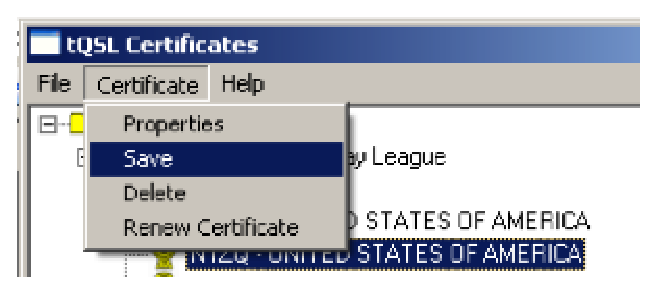
\includegraphics[width=0.5\textwidth]{savepkcs.eps}
		\caption{حفظ الشهادة المكتملة \textenglish{PKCS}}
		\label{fig:SavePKCS}
		\end{figure}
			قم بتحديد إشارة النداء ومن ثم اختر \textenglish{Certificate} من القائمة العلوية واختر \textenglish{Save}. يجب تحديد إشارة النداء لتتمكن من اختيار \textenglish{Certificate}. كما يمكنك الضغط على إشارة النداء بالزر الأيمن واختيار حفظ \textenglish{Save} كما هو موضح في الشكل \ref{fig:SavePKCS}.
		\item
			  سيقوم البرنامج بطلب تحديد كلمة مرور للملف \textenglish{p12} والخيار هنا لك. إن أردت
			  حفظ الملف بكلمة مرور فتأكد من كتابته في مكان آمن لأننا لن نتمكن من
			  مساعدتك في استرجاعها. وبدون كلمة المرور هذه لن تتمكن من استيراد ملف
			  الشهادة في حال تم تعطل جهازك.

	  		\begin{figure}[!hbtp]
	  		\centering
	  		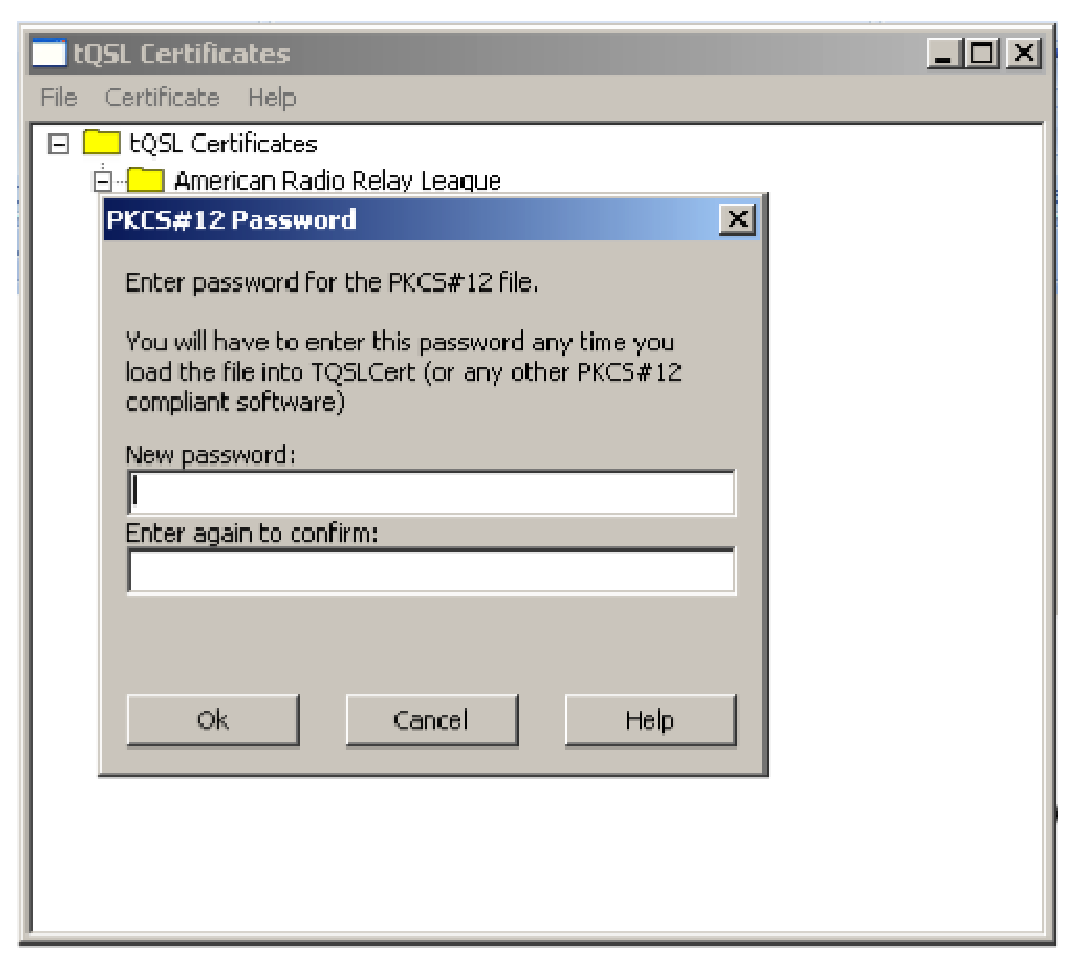
\includegraphics[width=0.5\textwidth]{pkcspassword.eps}
	  		\caption{لحفظ الشهادة بكلمة مرور}
	  		\label{fig:PKCSPassword}
	  		\end{figure}

			   وإن كنت قد اخترت حفظ المفتاح الشخصي
			  \textenglish{Private key} بواسطة كلمة مرور فيجب عليك إدخالها لفك الحماية عنها ولن
			  نتمكن من مساعدتك في حال فقدت كلمة المرور هذه أيضا فأنت الوحيد الذي
			  يعرفها. الرجاء التأكد من حفظ ملف الـ \textenglish{p12} في مكان غير جهاز الكمبيوتر
			  كقرص مدمج مثلا أو فلاش ميموري لأنه في حال حفظه على نفس الجهاز فلن
			  تستطيع الوصول له في حال تعطل الجهاز أو تمت سرقته!
	\end{enumerate}
	
\vspace{18pt}
\begin{center}
	\color{slategray2}
{\Huge \decoone}
\end{center}

\subsubsection{استيراد الشهادة\\}

\emph{ملاحظة: هذه الخطوات تُمَكِّنُك من استيراد ملف الشهادة بصيغة \textenglish{p12} على أي
من أجهزتك في المنزل أو المكتب أو غيرها سواء كانت تعمل على نظام
ويندوز أو ماك دون الحاجة للجهاز الذي تم إنشاء الملف عليه أو من خلاله.}

	\begin{enumerate}
		\item
		  قم بتنزيل برنامج \textenglish{Trusted QSL} على الجهاز الجديد.
		\item
		  قم بتشغيل برنامج \textenglish{TQSL Cert} بالضغط عليه مرتين من سطح المكتب من الأيقونة\ref{fig:Desktop2}.
		\item
		اختر \textenglish{Load Certificate File} كما هو موضح في الشكل \ref{fig:LoadTQ6}.
		\item
		\begin{figure}[!hbtp]
		\centering
		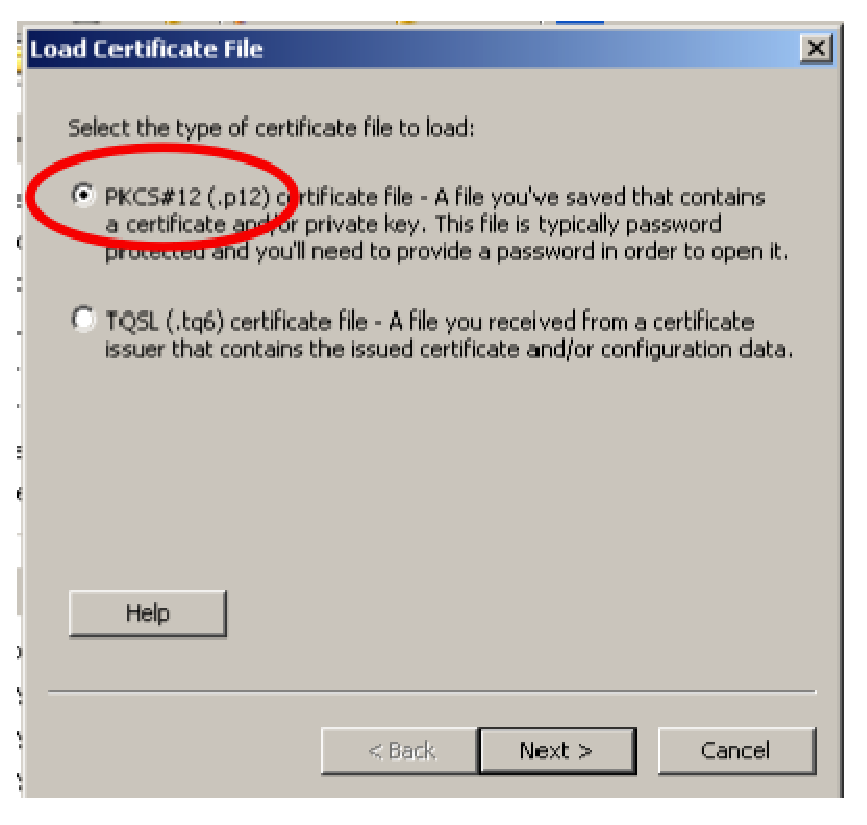
\includegraphics[width=0.5\textwidth]{pkcs.eps}
		\caption{الرجاء التأكد من اختيار \textenglish{PKCS}}
		\label{fig:SelectPKCS}
		\end{figure}
		  نوعية الملف المراد تحميله يجب أن تكون \textenglish{PKCS\#12} (\textenglish{p12}) بشكل إفتراضي.
		  الرجاء التأكد من ذلك كما هو موضح في الشكل \ref{fig:SelectPKCS}.
		\item
		  قم باختيار ملف الـ \textenglish{p12} من الفلاش ميموري أو قرص التخزين الخارجي أو
		  القرص المدمج أو من أي مكان آخر قمت بحفظه فيه.
		\item
		  سيطلب منك البرنامج كلمة المرور في حال قمت بحفظ الملف باستخدام كلمة
		  مرور.
		\item
		  قم بالضغط على \textenglish{Finish} في أسفل صندوق تقرير تحميل الشهادة. ستجد الآن
		  شريطة ذهبية بجانب إشارة نِدائِك في نافذة برنامج \textenglish{TQSL Cert} كما هو موضح في الشكل \ref{fig:SignedTQ6}.
		\item
		  بإمكانك الآن إنشاء موقع المحطة الجغرافي في برنامج \textenglish{TQSL}.
	\end{enumerate}

بهذا نكون قد أتممنا عملية التعامل مع الشهادات و بإمكانك طلب شهادات إشارة
نداء إضافية لإشاراة النداء السابقة أو المُتَنَقّلَة والمرتبطة بك من خلال طلب
ورفع شهادة إشارة نداء مختومة لكل إشارة نداء.

% end of section
\vspace{24pt}
\begin{center}
	\color{slategray2}
{\Huge\hrulefill\hspace{0.2cm} \floweroneright\floweroneleft \hspace{0.2cm} \hrulefill}
\end{center}
\newpage


\section{الخطوة الخامسة - إنشاء الموقع الجغرافي للمحطة}

الموقع الجغرافي للمحطة يحتوى على كل البيانات الجغرافية المطلوبة. ويتضمن
ذلك منطقة الـ {\href{http://www.mapability.com/ei8ic/maps/ituzone.php}{\textenglish{ITU}}\footnote{تقسيم \textenglish{ITU} للمناطق.}} والـ {\href{http://www.mapability.com/ei8ic/maps/cqzone.php}{\textenglish{CQ}}}\footnote{تقسيم CQ للمناطق.} و موقع التقاطع الشبكي واسم الولاية والمقاطعة
ورقم الأيوتا \textenglish{IOTA}\footnote{الأيوتا \textenglish{IOTA} هي اختصار للجملة \textenglish{Island On The Air} وهي منظمة تهتم بإحياء الجُزُر المَيّتة من خلال إقامة فعاليات معينة.} إن كنت تعمل من جزيرة.

الرجاء التأكد من إكتمال البيانات بشكل دقيق عند إدخالها في هذه الخطوة حيث
أنها الطريقة الوحيدة لتأكيد موقعك من قِبَل أي محطة تقوم بعمل إتصال \textenglish{QSO}
معك.

\vspace{18pt}
\begin{center}
	\color{slategray2}
{\Huge \decoone}
\end{center}

\subsection{تفاصيل إنشاء الموقع الجغرافي للمحطة}

بما أنك قمت بالحصول على الشهادة الإلكترونية والتي تخولك ختم ورفع دفتر
سجلاتك إلى دفتر سجلات العالم \textenglish{Loogbook of The World} فإن أول خطوة في عملية
الختم هي إنشاء الموقع الجغرافي للمحطة. هذا الموقع يحتوي على معلومات
جغرافية حول محطتك ويتضمن ذلك المنطقة وموقع التقاطع الشبكي ورقم الأيوتا
\textenglish{IOTA} والولاية والدولة.

الرجاء التأكد من إكتمال البيانات بشكل دقيق وكامل عند إدخالها في هذه
الخطوة حيث أنها الطريقة الوحيدة لتأكيد موقعك من قبل أي محطة تقوم بعمل
إتصال \textenglish{QSO} معك.

	\begin{enumerate}
		\item
			\begin{figure}[!hbtp]
			\centering
			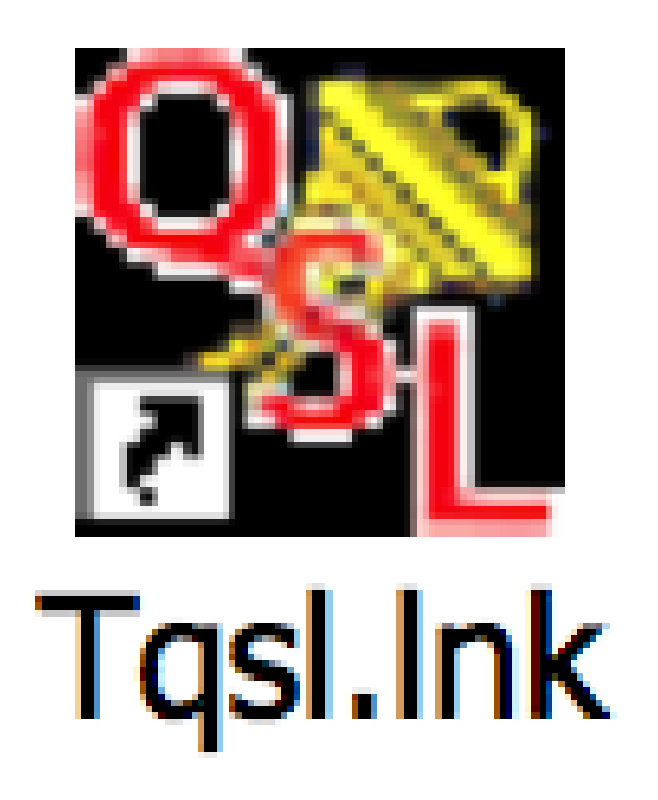
\includegraphics[width=0.1\textwidth]{tqsl.eps}
			\caption{برنامج TQSL}
			\label{fig:TQSL}
			\end{figure}
			  قم بفتح برنامج \textenglish{TQSL} كما هو موضح في الشكل \ref{fig:TQSL}.
\clearpage
		\item
			\begin{figure}[!hbtp]
			\centering
			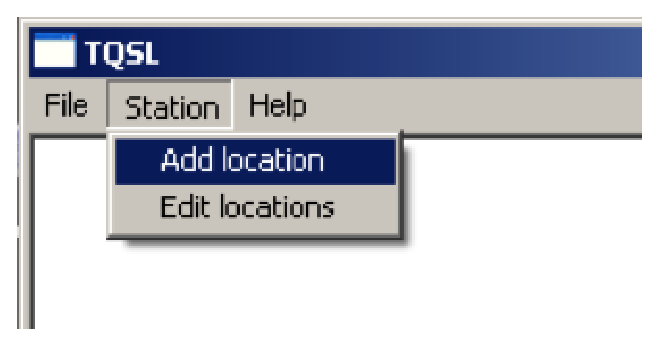
\includegraphics[width=0.4\textwidth]{locationadd.eps}
			\caption{إضافة موقع جديد}
			\label{fig:LocationAdd}
			\end{figure}
			  اختر \textenglish{Station} ومن ثم \textenglish{Add Location} كما هو موضح في الشكل \ref{fig:LocationAdd}.
		\item
			\begin{figure}[!hbtp]
			\centering
			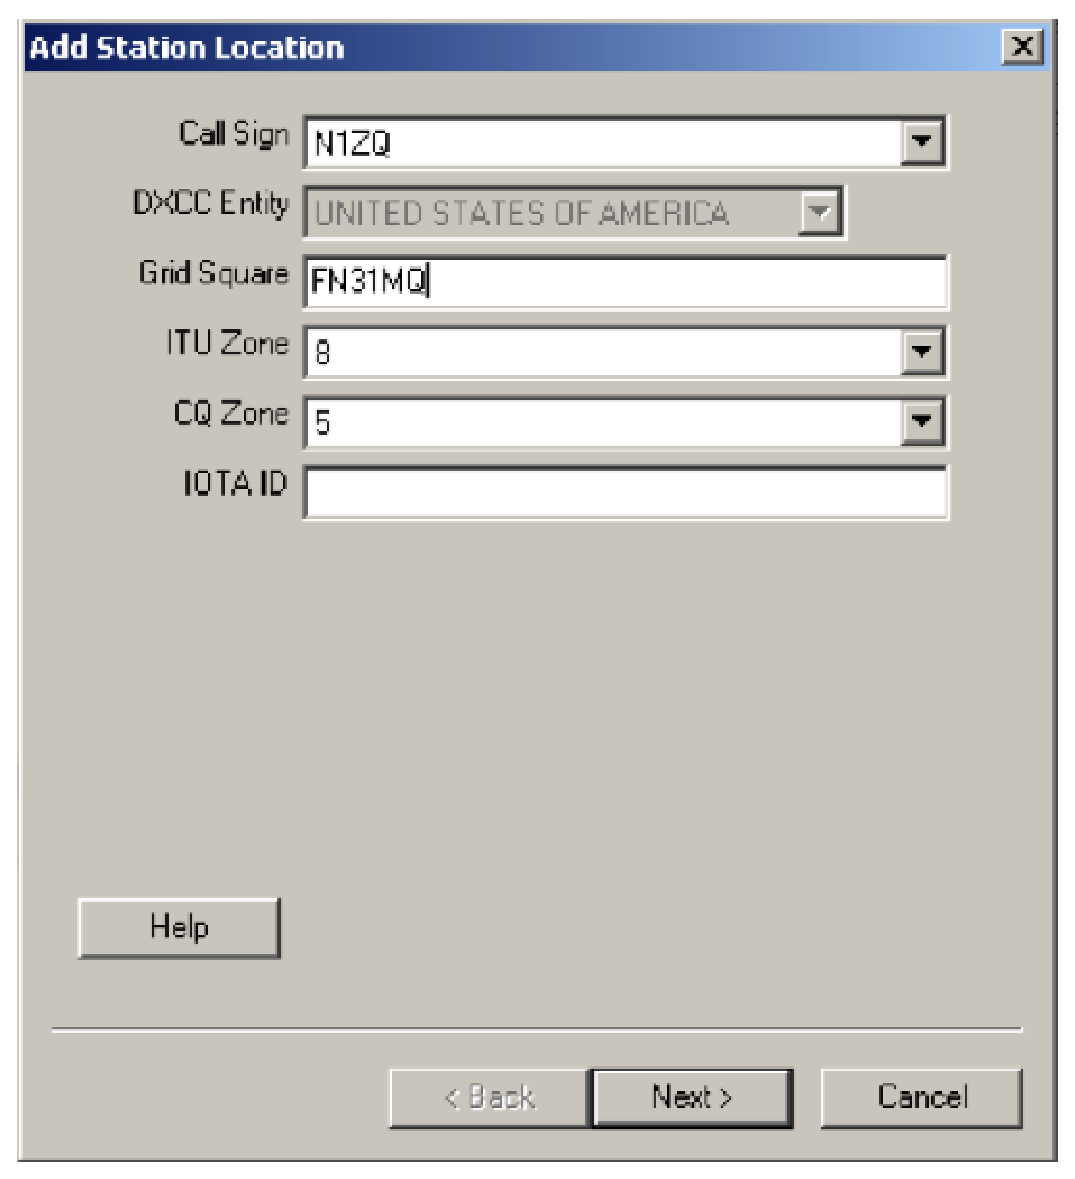
\includegraphics[width=0.48\textwidth]{locationinfo.eps}
			\caption{بيانات موقع المحطة الخاصة بك}
			\label{fig:LocationInfo}
			\end{figure}
			  قم بتعبئة الخانات المطلوبة كما هو موضح في الشكل \ref{fig:LocationInfo}.
  		\item
			\begin{figure}[!hbtp]
			\centering
			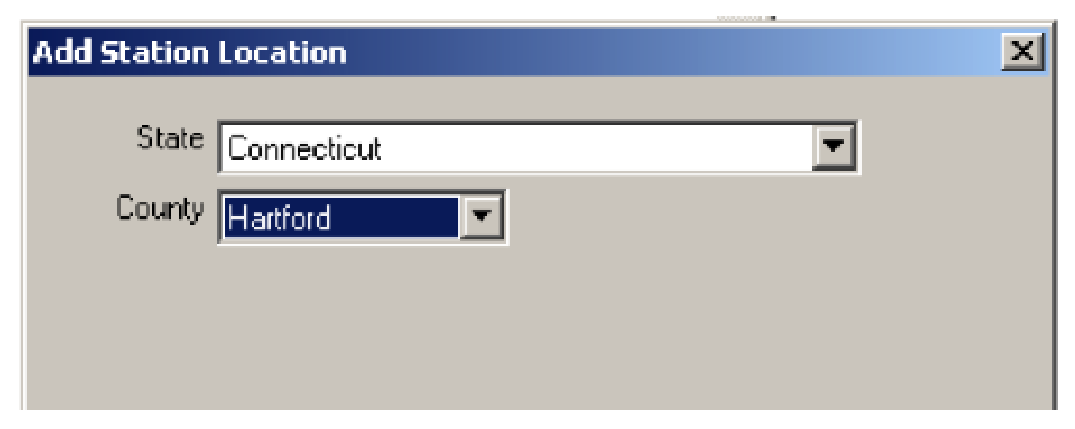
\includegraphics[width=0.48\textwidth]{locationstate.eps}
			\caption{اختر الولاية والمقاطعة الأمريكية التي تُقيم بها إن كنت تحمل إشارة نداء أمريكية}
			\label{fig:LocationState}
			\end{figure}
			صاحب إشاراة النداء الأمريكية بإمكانه اختيار الولاية والمقاطعة التي يُقيم بها من القائمة المُنسَدلة كما هو موضح في الشكل \ref{fig:LocationState}.
		\item
			\begin{figure}[!hbtp]
			\centering
			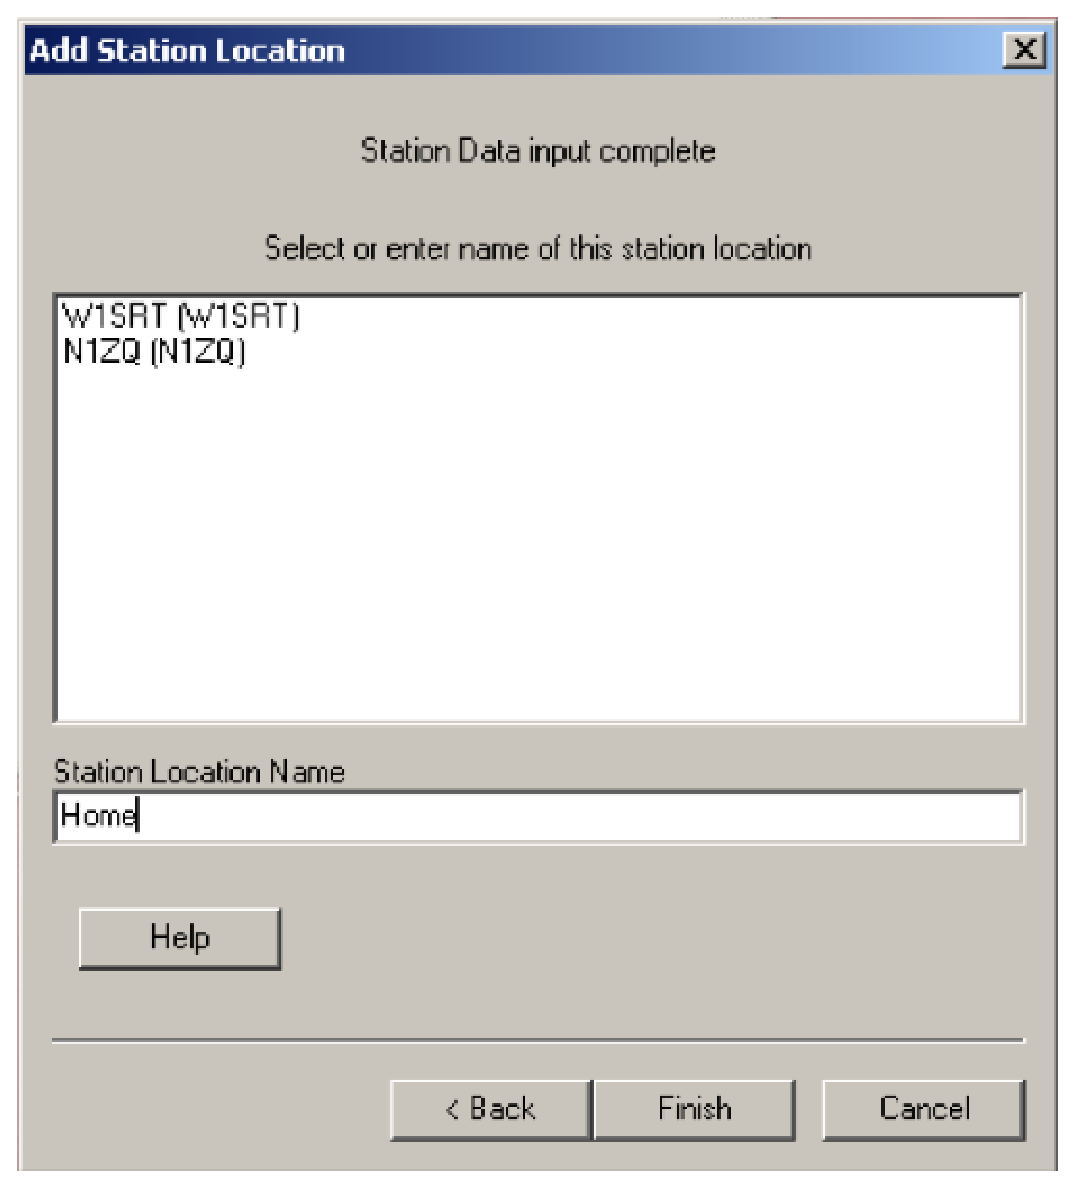
\includegraphics[width=0.48\textwidth]{locationname.eps}
			\caption{الاسم الخاص بالموقع}
			\label{fig:LocationName}
			\end{figure}
			  آخر خطوة هي لتسمية الموقع الجغرافي والذي قد يكون \textenglish{Home} أي المنزل مثلا
		  ثم اضغط \textenglish{Finish} كما هو موضح في الشكل \ref{fig:LocationName}.
	\end{enumerate}


% end of section
\vspace{24pt}
\begin{center}
	\color{slategray2}
{\Huge\hrulefill\hspace{0.2cm} \floweroneright\floweroneleft \hspace{0.2cm} \hrulefill}
\end{center}
\newpage


\section{الخطوة السادسة - ختم ورفع ملفات دفتر السجلات}

دفتر سجلات العالم يقبل ملفات الـ \textenglish{Trusted QSL} والتي تم ختمها إلكترونيا.
وقد قمنا باستخدامها مسبقا أثناء إنشاء شهادة إشارة النداء \textenglish{TQ5} و \textenglish{TQ6}.

عندما تقوم بختم دفتر السجلات الخاص بك سواء كان بصيغة \textenglish{ADIF}\footnote{نَسْق تبادل بيانات الهواة {\href{http://www.adif.org/adif302.htm}{http://www.adif.org/adif302.htm}}} أو \textenglish{Cabrillo}\footnote{هي أدارة ربط \textenglish{interface} بين برنامج دفتر السجلات و رعاة المسابقات لتسهيل عملية تجميع بيانات المسابقات ونتائجها تلقائيا. {\href{http://www.kkn.net/~trey/cabrillo/faq.txt}{http://www.kkn.net/~trey/cabrillo/faq.txt}}}
فإنك حقيقة تقوم بعمل ملف جديد باسم ملف \textenglish{TQ8}. والبيانات الموجودة في هذا
الملف هي ذاتها التي تتواجد في أي بطاقة تأكيد الإتصال \textenglish{QSL Cards}\footnote{وهي بطاقات تأكيد الإتصال بين الهواة.}. كما سيتم
استيراد إشارة ندائك وموقعك حسب تقسيم \textenglish{DXCC} من شهادة إشارة النداء بينما
بيانات الإتصال سيتم جلبها من ملف دفتر السجلات المستخدَم. أضف إلى ذلك أن
جميع البيانات المتعلقة بموقع محطتك الجغرافي سيتم جلبه من الموقع الجغرافي
للمحطة في برنامج \textenglish{TQSL}.

بعض البرامج الخاصة بتخزين بيانات دفتر السجلات تتميز بخاصية وجود إختصار
لعملية ختم دفتر السجل و رفعه. لذلك يفضل التأكد من البرنامج الذي تستخدمه
في حفظ دفتر السجلات أو مراسلة مطور البرنامج عن هذه الخاصية.

ختم دفتر السجلات لن يأخذ أكثر من بضع نقرات بالفأرة.

\vspace{18pt}
\begin{center}
	\color{slategray2}
{\Huge \decoone}
\end{center}

\subsection{تفاصيل ختم ورفع ملفات دفتر السجلات}

ستتمكن من ختم دفتر سجلاتك إلكترونيا في هذه الخطوة وسينتج عن ذلك
ملف مختوم إلكترونياً اسمه \textenglish{TQ8} وهو المطلوب رفعه إلى \textenglish{LoTW}.

يجب أولا تصدير دفتر سجلاتك من البرنامج الذي تستخدمه بصيغة \textenglish{ADIF}
أو \textenglish{Cabrillo} وقد تقوم بعض البرامج المتطورة بعمل هذه الخطوة لك تلقائيا.
تأكد من البرنامج الذي تستخدمه لحفظ دفتر السجلات.

	\begin{enumerate}
		\item
			\begin{figure}[!hbtp]
			\centering
			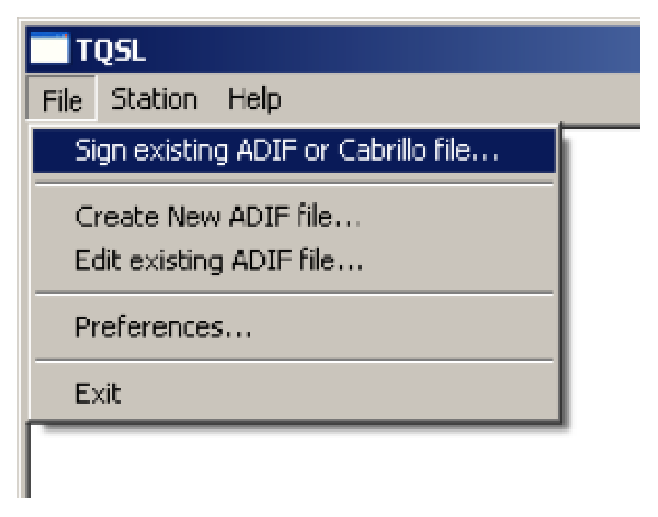
\includegraphics[width=0.30\textwidth]{signnew.eps}
			\caption{اختيار ختم دفتر سجلات}
			\label{fig:SignNew}
			\end{figure}
			بعد تشغيل برنامج \textenglish{TQSL} قم باختيار \textenglish{File} ومن ثم اختر \textenglish{Sign existing ADIF or Cabrillo file\ldots{}} كما هو موضح في الشكل \ref{fig:SignNew}.
\clearpage
		\item
			\begin{figure}[!hbtp]
			\centering
			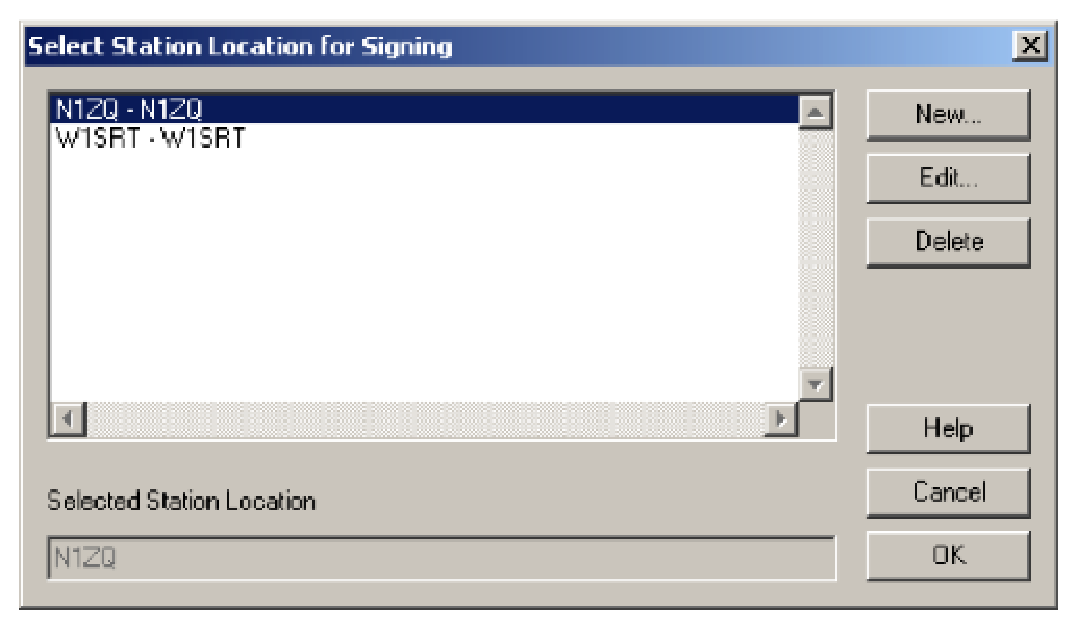
\includegraphics[width=0.48\textwidth]{signselectstation.eps}
			\caption{تأكد من اختيار المحطة الصحيحة لختم دفتر السجلات}
			\label{fig:SignStation}
			\end{figure}
		  اختر الموقع الجغرافي للمحطة لاستخدامه مع دفتر السجلات من خلال تحديد
		  الموقع ومن ثم الضغط على \textenglish{OK} كما هو موضح في الشكل \ref{fig:SignStation}.

		\item
			\begin{figure}[!hbtp]
			\centering
			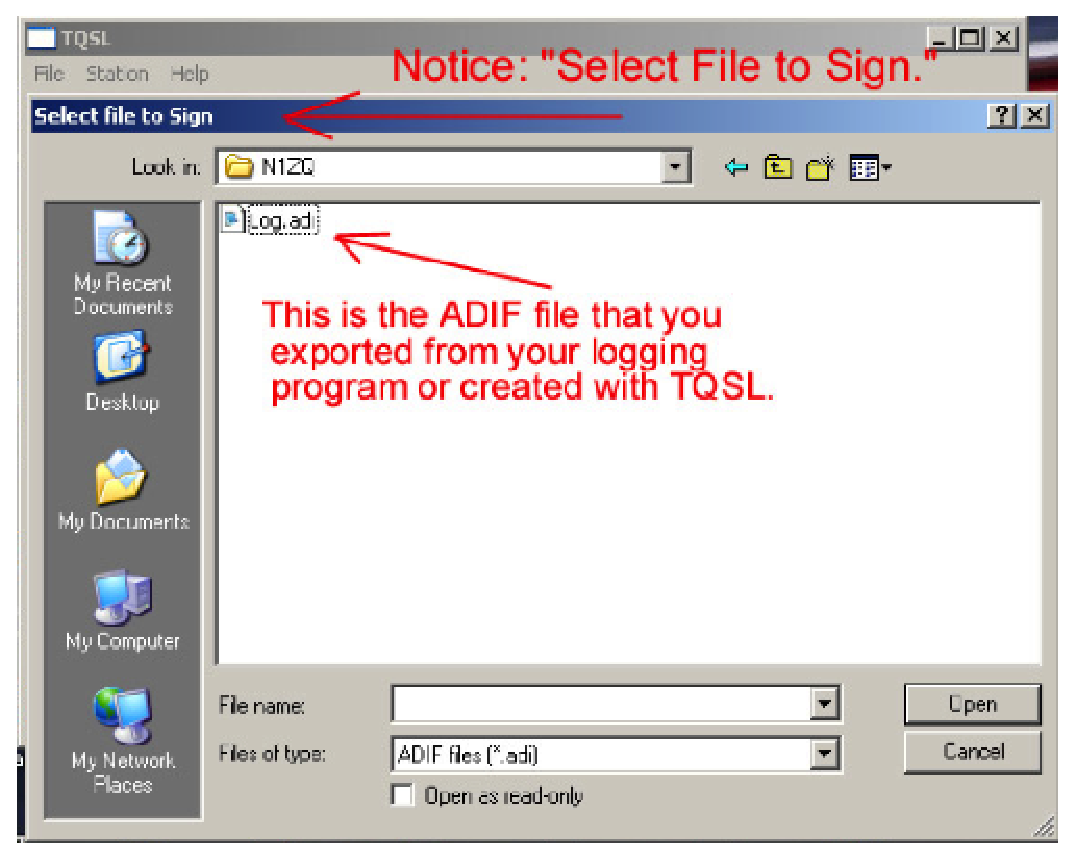
\includegraphics[width=0.58\textwidth]{signselectfiletosign.eps}
			\caption{تأكد من اختيار ملف دفتر السجلات الصحيح المراد ختمه}
			\label{fig:SignFileToSign}
			\end{figure}
		  اختر ملف دفتر السجلات المراد ختمه إلكترونيا ومن ثم اختر فتح \textenglish{Open} كما هو موضح في الشكل \ref{fig:SignFileToSign}. يُفضل
		  استخدام اسم فريد في كل مرة تقوم بتصدير الملف فيها لمساعدتك في متابعة
		  ذلك.
\clearpage
		\item
			\begin{figure}[!hbtp]
			\centering
			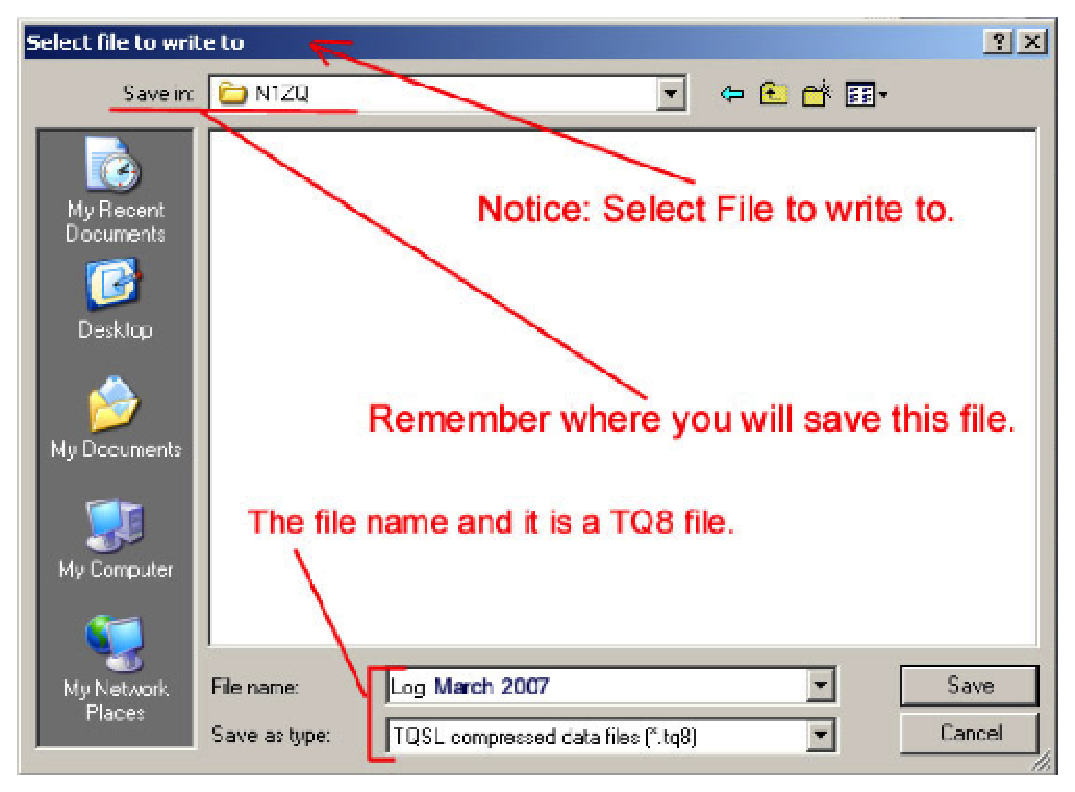
\includegraphics[width=0.58\textwidth]{signselectfiletowrite.eps}
			\caption{تأكد من تحديد الموقع الصحيح لحفظ الملف}
			\label{fig:SignFileToWrite}
			\end{figure}
		  قم بتحديد الموقع المراد حفظ الملف الجديد (ملف \textenglish{TQ8}) فيه كما هو موضح في الشكل \ref{fig:SignFileToWrite}. وعند ختم ملف
		  دفتر السجلات إلكترونيا ينتج عنه ملف مشفر بصيغة \textenglish{TQ8} وهو الملف المطلوب
		  رفعه إلى \textenglish{LoTW}.
		\item
			\begin{figure}[!hbtp]
			\centering
			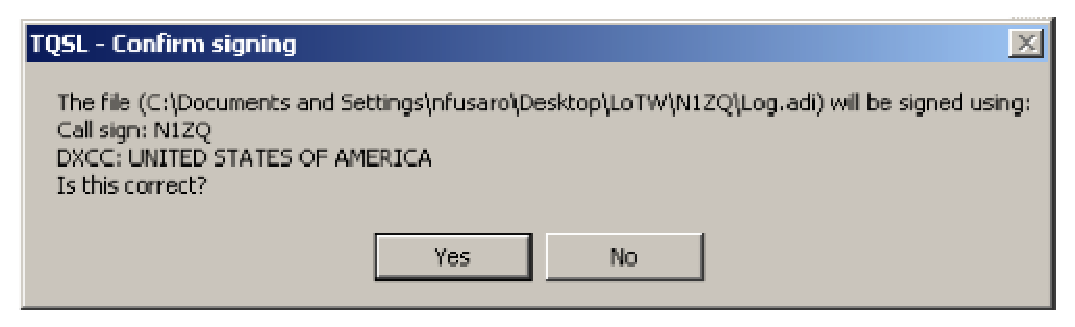
\includegraphics[width=0.5\textwidth]{signconfirmation.eps}
			\caption{نافذة تأكيد ختم الملف}
			\label{fig:SignConfirm}
			\end{figure}
		  ستظهر نافذة تأكيد ختم الملف كما هو موضح في الشكل \ref{fig:SignConfirm}. علما أنه في حال وجود أكثر من إشارة نداء
		  على الجهاز فيجب عليك التأكد من أنك تقوم بختم الملف بإشارة النداء
		  الصحيحة.
\clearpage
		\item
			\begin{figure}[!hbtp]
			\centering
			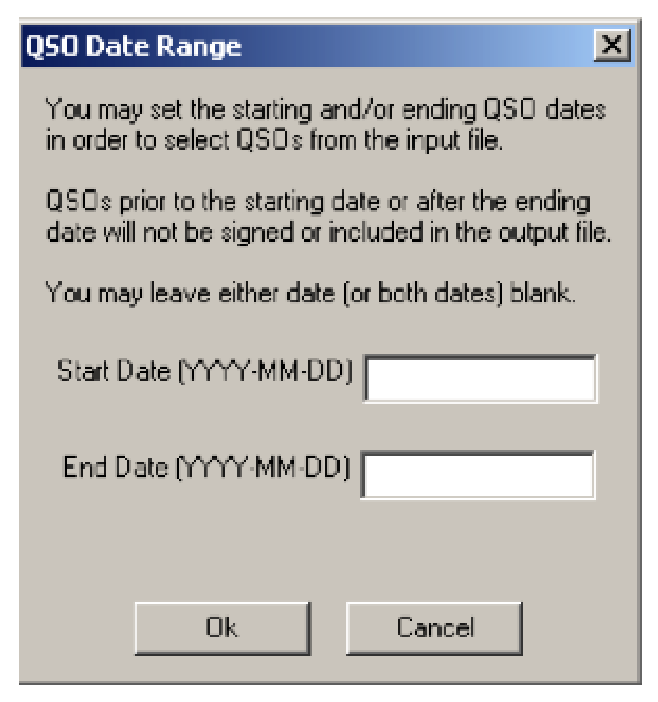
\includegraphics[width=0.4\textwidth]{signqsodaterange.eps}
			\caption{نافذة تاريخ الإتصالات}
			\label{fig:SignQSODate}
			\end{figure}
		  بمقدورك تحديد نطاق لتاريخ الإتصالات كما يمكنك تركه فارغا لأنه في حال
		  وجود معلومات مكررة فإن الموقع سيُبقي على البيانات الأحدث كما هو موضح في الشكل \ref{fig:SignQSODate}. علما أنه يُفضل
		  تحديد تاريخ آخر رفع على موقع \textenglish{LoTW} كتاريخ للبداية \textenglish{beginning date}.
		\item
		  سيبين لك البرنامج تحويل البيانات الُمدخلة في دفتر السجلات إلى صيغة
		  \textenglish{TQSL} المطلوبة ومن ثم ستظهر لك رسالة بأن الملف \textenglish{TQ8} جاهز وبإمكانك رفعه.
		\item
			  قم بتسجيل الدخول إلى موقع \href{https://p1k.arrl.org/lotwuser/default}{\textenglish{LoTW}}.
\clearpage
		\item
			\begin{figure}[!hbtp]
			\centering
			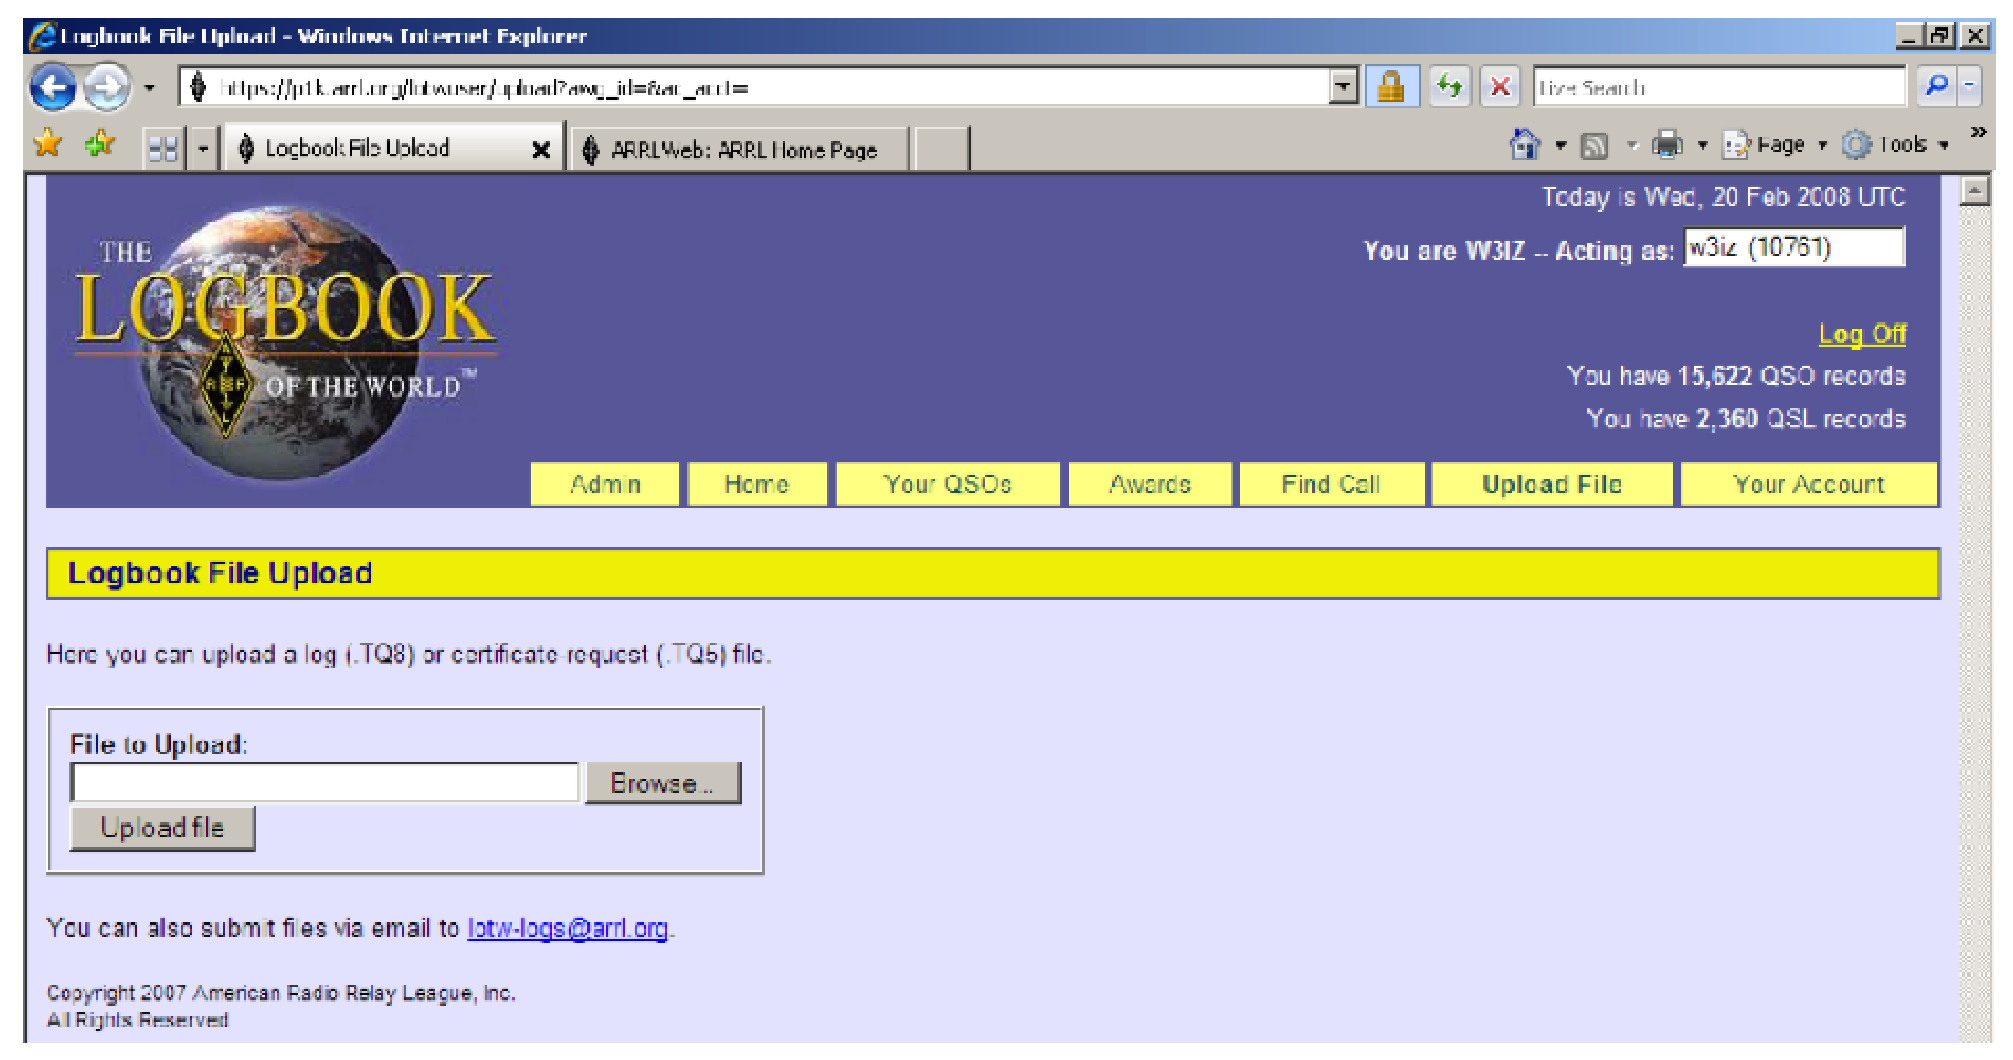
\includegraphics[width=1.0\textwidth]{signlotw.eps}
			\caption{صفحة \textenglish{LoTW} بعد اختيار تبويبة \textenglish{Upload File}}
			\label{fig:SignLoTW}
			\end{figure}
		  قم باختيار تبويبة \textenglish{Upload File} كما هو موضح في الشكل \ref{fig:SignLoTW}.
		\item
		  استخدم زر تصفح \textenglish{Browse} لاختيار ملف \textenglish{TQ8} من جهازك.
		\item
		  قم بالضغط على \textenglish{Upload file} لرفع الملف. ستظهر لك رسالة بأنه تتم معالجة الملف
		  في حال تمت عملية الرفع بنجاح.
	\end{enumerate}

أما في حال استلامك لرسالة مثل: \textenglish{FILE does not appear to be a
TrustedQSL file! Processing aborted} فيبدو أنك قمت باختيار ملف خاطيء أو لم تقم باختيار ملف \textenglish{TQ8} المناسب.

% end of section
\vspace{24pt}
\begin{center}
	\color{slategray2}
{\Huge\hrulefill\hspace{0.2cm} \floweroneright\floweroneleft \hspace{0.2cm} \hrulefill}
\end{center}

\vspace{30pt}
\center{\huge{شكرا لاستخدامك دفتر سجلات العالم \\\textenglish{Logbook of The World}}}

\newpage
\listoffigures\newpage

\end{document}